\chapter{Scaling up Gaussian Process Regression}
\label{chapScalingGPR}


\begin{mdframed}[hidealllines=true,backgroundcolor=lightgray!20]
\section*{Résumé}
Le calcul de distributions postérieures dans les GPs devient difficile pour les ensembles de données de la grosse taille. Le calcul de la matrice de précision est une opération de complexité $ \mathcal{O}(N ^ {3}) $, mettant une limite de $ N \sim 10^4 $ points de données pour la construction de modèles. Ce chapitre décrit l'état de l'art pour l'étendue des GPs pour les tâches de régression. Il existe deux methodes pour étendre des GPs, la première méthode 'Sparse GPs' utilisent un ensemble des points inductifs pour réduire le coût de calcul de la matrice de précision. La seconde est appelée `Distributed GP ' elle divise l'ensemble de données en sous-ensembles plus petits, en distribuant le modèle en plusieurs lots.

Les méthodes `Sparse GPs 'utilisent le approximation de Nystr\"{o}m, récrivant la matrice de Gram comme l'équation \ref{subSecSamplingFunctionsGPPrior}, diminuant ainsi la complexité de calcul à $ \mathcal{O} (NM^{2}) $ (M $ \ll $ N) , $ M $ étant le nombre de points inductifs. Grâce à des expériences sur les données synthétiques, on peut montrer que on peut fixer $ M \sim N/10 $ quand les points inductifs sont distribués alétoirement et $ M \sim N/50 $ quand les emplacements des points inductifs sont optimisés. Cette approximation pousse la limite de régression GP à $ N \sim 10^6 $ points de données.

«Distributed GPs» distribue les tâches de régression GP dans plusieurs lots, diminuant ainsi la complexité informatique à $ \mathcal{O} (NP^{3}) $ (P $\ll$ N), $ P $ étant le nombre (numéro) des points dans un lot. Grâce à des expériences sur les données synthétiques, nous démontrons que $ P \sim N/100 $ n'affecte pas beaucoup la précision de la régression. En fait, nous pouvons réduire davantage $ P $ si nous permettons la répétition de points entre les lots. Cela permet d'étendre le GP à n'importe quel nombre de points de données.
\end{mdframed}


%\pagebreak

\section{Introduction}
The GP regression approach, as mentioned in earlier chapter, is intractable for large data sets. For a data set of size $N$ the covariance matrix $\myMatrix{K_{XX}}$ is of size $N \times N$ and $\mathcal{O}\left ( N^{3} \right )$ time is needed for calculating the precision matrix and $\mathcal{O}\left ( N^{2} \right )$ memory for storage. Since inverting the covariance matrix takes considerable amount of time and memory, almost all techniques to scale up GP regression try to approximate the inversion of Gram matrix $\myMatrix{K_{XX}}$. 

Let us take the example of a SE kernel, for a large value of length-scale, the Gram matrix ( $\myMatrix{K_{XX}}$) is spread out and has a rank lower than  $N$ (figure \ref{subFigSEPrior_2}). Due to this characteristic, the Gram matrix can be approximated using low-rank approximations, reducing the cost of inverting the Gram matrix. In the GP literature, sparse approximations (section \ref{secSparseApprox}) use a set of inducing points to compress the information of the several observations through the low-rank approximation. 

For the same SE kernel, if the length-scale tends to a low value, the Gram matrix is not of low-rank but tends to a diagonal matrix (figure \ref{subFigSEPrior_1}). In the GP literature the mixture of experts (section \ref{secDgp}) methodology exploits the block diagonal nature of the Gram matrix by distributing data points into a subset of experts, assuming independence across experts and distributing the calculations into several batches. The first regime suggests global (numerical) low-rank approximations while the second regime suggests local block-diagonal approximations \cite{march2015askit, chenhan2016inv}. 

The remaining chapter unfolds as follows, section \ref{secSparseApprox} describes the Sparse Approximations detailing several methods of choosing inducing points and then performing experiments on a toy dataset. Section \ref{secDgp} describes the Distributed GP methodology detailing several methods for merging of experts and then performing experiments on the same toy-dataset. 

\section{Sparse Approximations}\label{secSparseApprox}
Sparse methods use a small subset of input points as support or inducing points to approximate the Gram matrix. Suppose we use $M$ inducing points $\myMatrix{X^{m}} = \{\VEC{x^{m}_{1}}, \VEC{x^{m}_{2}}, \ldots, \VEC{x^{m}_{M}}\}^T$, such that $M < N$. The points $\myMatrix{X^{m}}$ can be a subset of training inputs in the input space. 


\subsection{Nystr\"{o}m Approximation}\label{subSecNystrom} 

Using Nystr\"{o}m approximation the Gram matrix can be approximated as equation \ref{eqnSparseNystormGram} \cite{quinonero2005unifying, seeger2003fast}, for more detail refer to \cite{williams2001using}. 

\begin{equation}\label{eqnSparseNystormGram}
\myMatrix{K_{Nystorm}(X, X)} = \myMatrix{K(X, X^{m})} \myMatrix{K(X^{m}, X^{m})}^{-1} \myMatrix{K(X^{m}, X)}
\end{equation}

Here, $\myMatrix{K(X^{m}, X^{m})}$ is a $M \times M$ Gram matrix evaluated at inducing points $\myMatrix{X^{m}}$, $\myMatrix{K(X, X^{m})}$ is an $N \times M$ Gram matrix between training points and inducing points. The inversion of approximate matrix takes $\mathcal{O}\left ( NM^{2} \right )$ time to compute. The code \ref{codeGramNystrom} defines a function `evaluateNystromGramMatrix' which is used to evaluate the Nstr\"{o}m approximation of the Gram matrix. 

\begin{mdframed}[hidealllines=true,backgroundcolor=lightgray!20]
\lstinputlisting[caption={Gram Matrix using Nystr\"{o}m Approximation}, 
                    captionpos=b, 
                    label={codeGramNystrom}, 
                    backgroundcolor = \color{MatlabCellColour},
                    style=Matlab-editor,
                    basicstyle=\color{black}\ttfamily\small]
                    {codes/chapter3/evaluateNystromGramMatrix.m}
\end{mdframed}


Figure \ref{subFigNystormSEmatrix} is an approximate Gram matrix computation using Nystr\"{o}m approximation of the matrix in figure \ref{subFigcovSEmatrix_1} at the input points $\myMatrix{X^{*}} = \{[0:0.02:1]\}$. The inducing points $\myMatrix{X^{m}}$ are chosen randomly from the set of input points and their location is denoted by white lines. We can observe that if the gap between inducing points increases, the accuracy of the Gram matrix degrades (eg. at $x \sim 0.5$). Figure \ref{subFignystormSEmatrixUniform} is again an approximated Gram matrix using Nystr\"{o}m approximation of the matrix in figure \ref{subFigcovSEmatrix_1}. This time the equally spaced inducing points are chosen in the range of $\myMatrix{X^{*}}$. Notice the significant improvement in the Gram matrix upon different set of inducing inputs.

\begin{figure}[!ht]
  \centering
    \subfigure[{Approximated Gram matrix using Nystr\"{o}m approximation for a SE Kernel with $(\VEC{\theta} = [1, 0.2])$ (figure \ref{subFigcovSEmatrix_1}) at the input points $\myMatrix{X^{*}} = \{[0:0.02:1]\}$. The inducing points were chosen randomly, the white lines denote the location of inducing points. }]
  {
        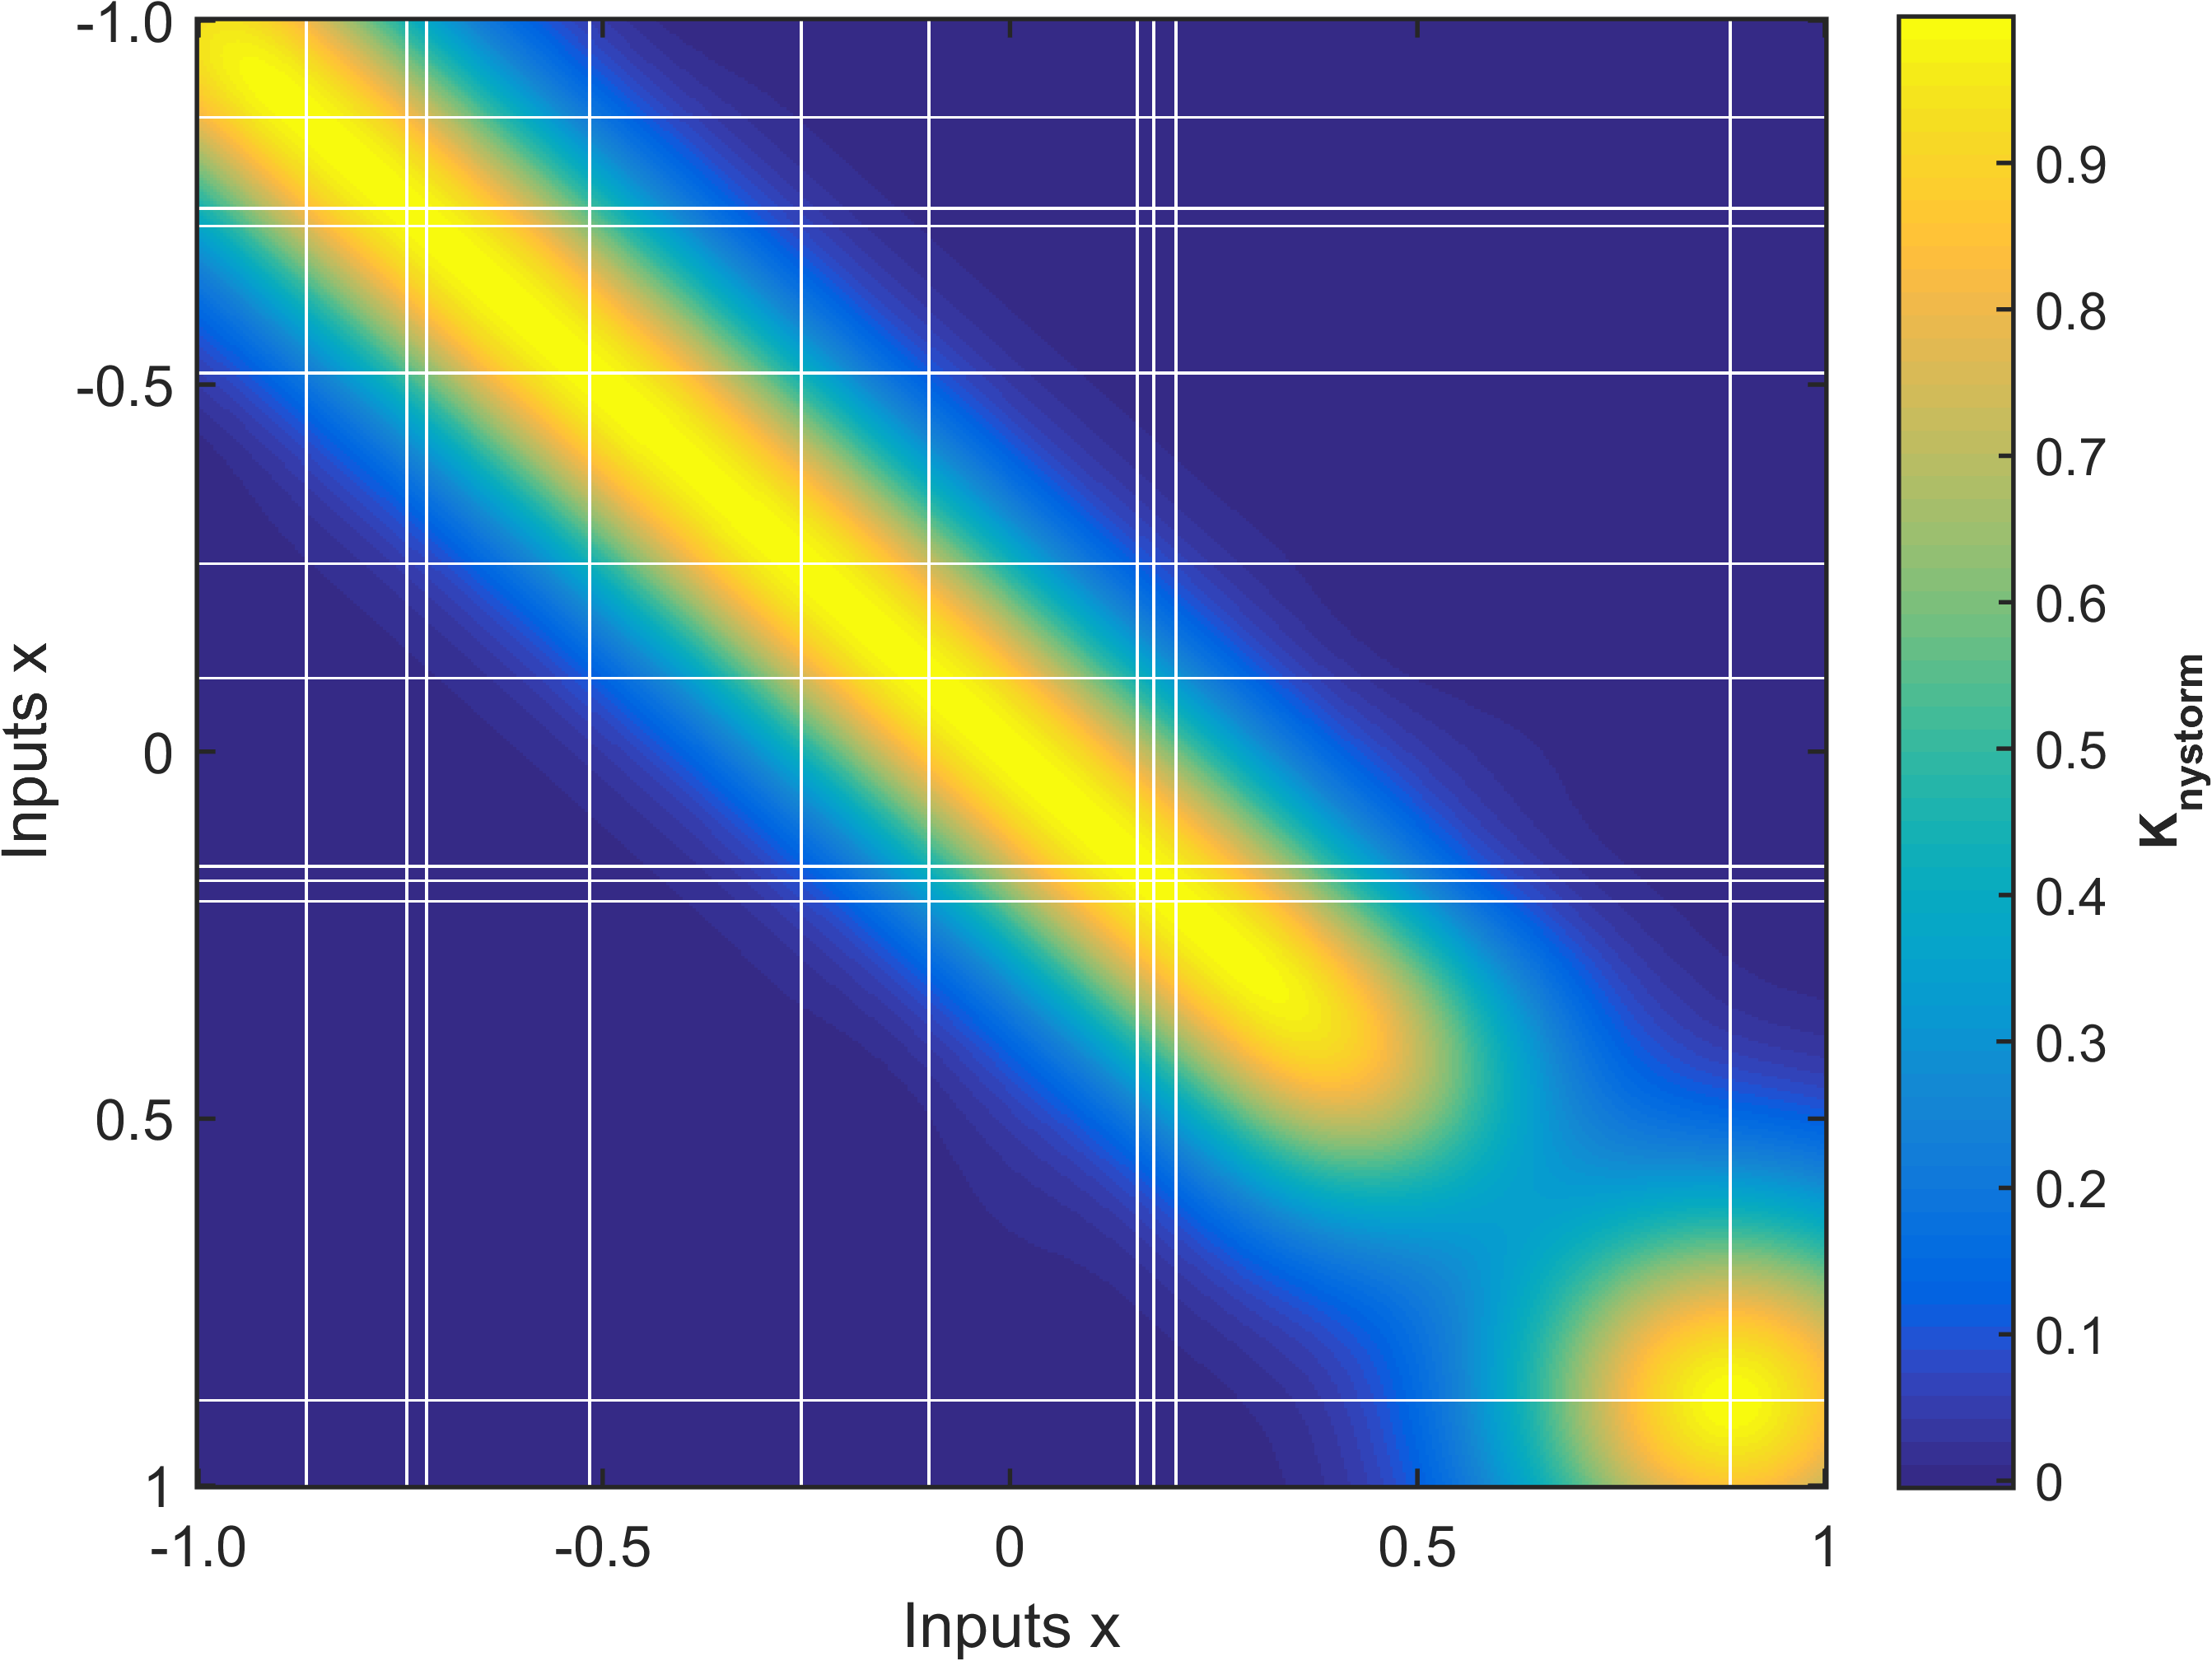
\includegraphics[width=0.45\textwidth]
        {images/part1/nystormSEmatrix}
        \label{subFigNystormSEmatrix}
  }\quad
\subfigure[{Approximated Gram matrix using Nystr\"{o}m approximation for a SE Kernel with $(\VEC{\theta} = [1, 0.2])$ (figure \ref{subFigcovSEmatrix_1}) at the input points $\myMatrix{X^{*}} = \{[0:0.02:1]\}$. The white lines denote the location of inducing points, the inducing points are uniformly distributed. Notice the significant improvement in Gram matrix due to different inducing inputs}]
  {
        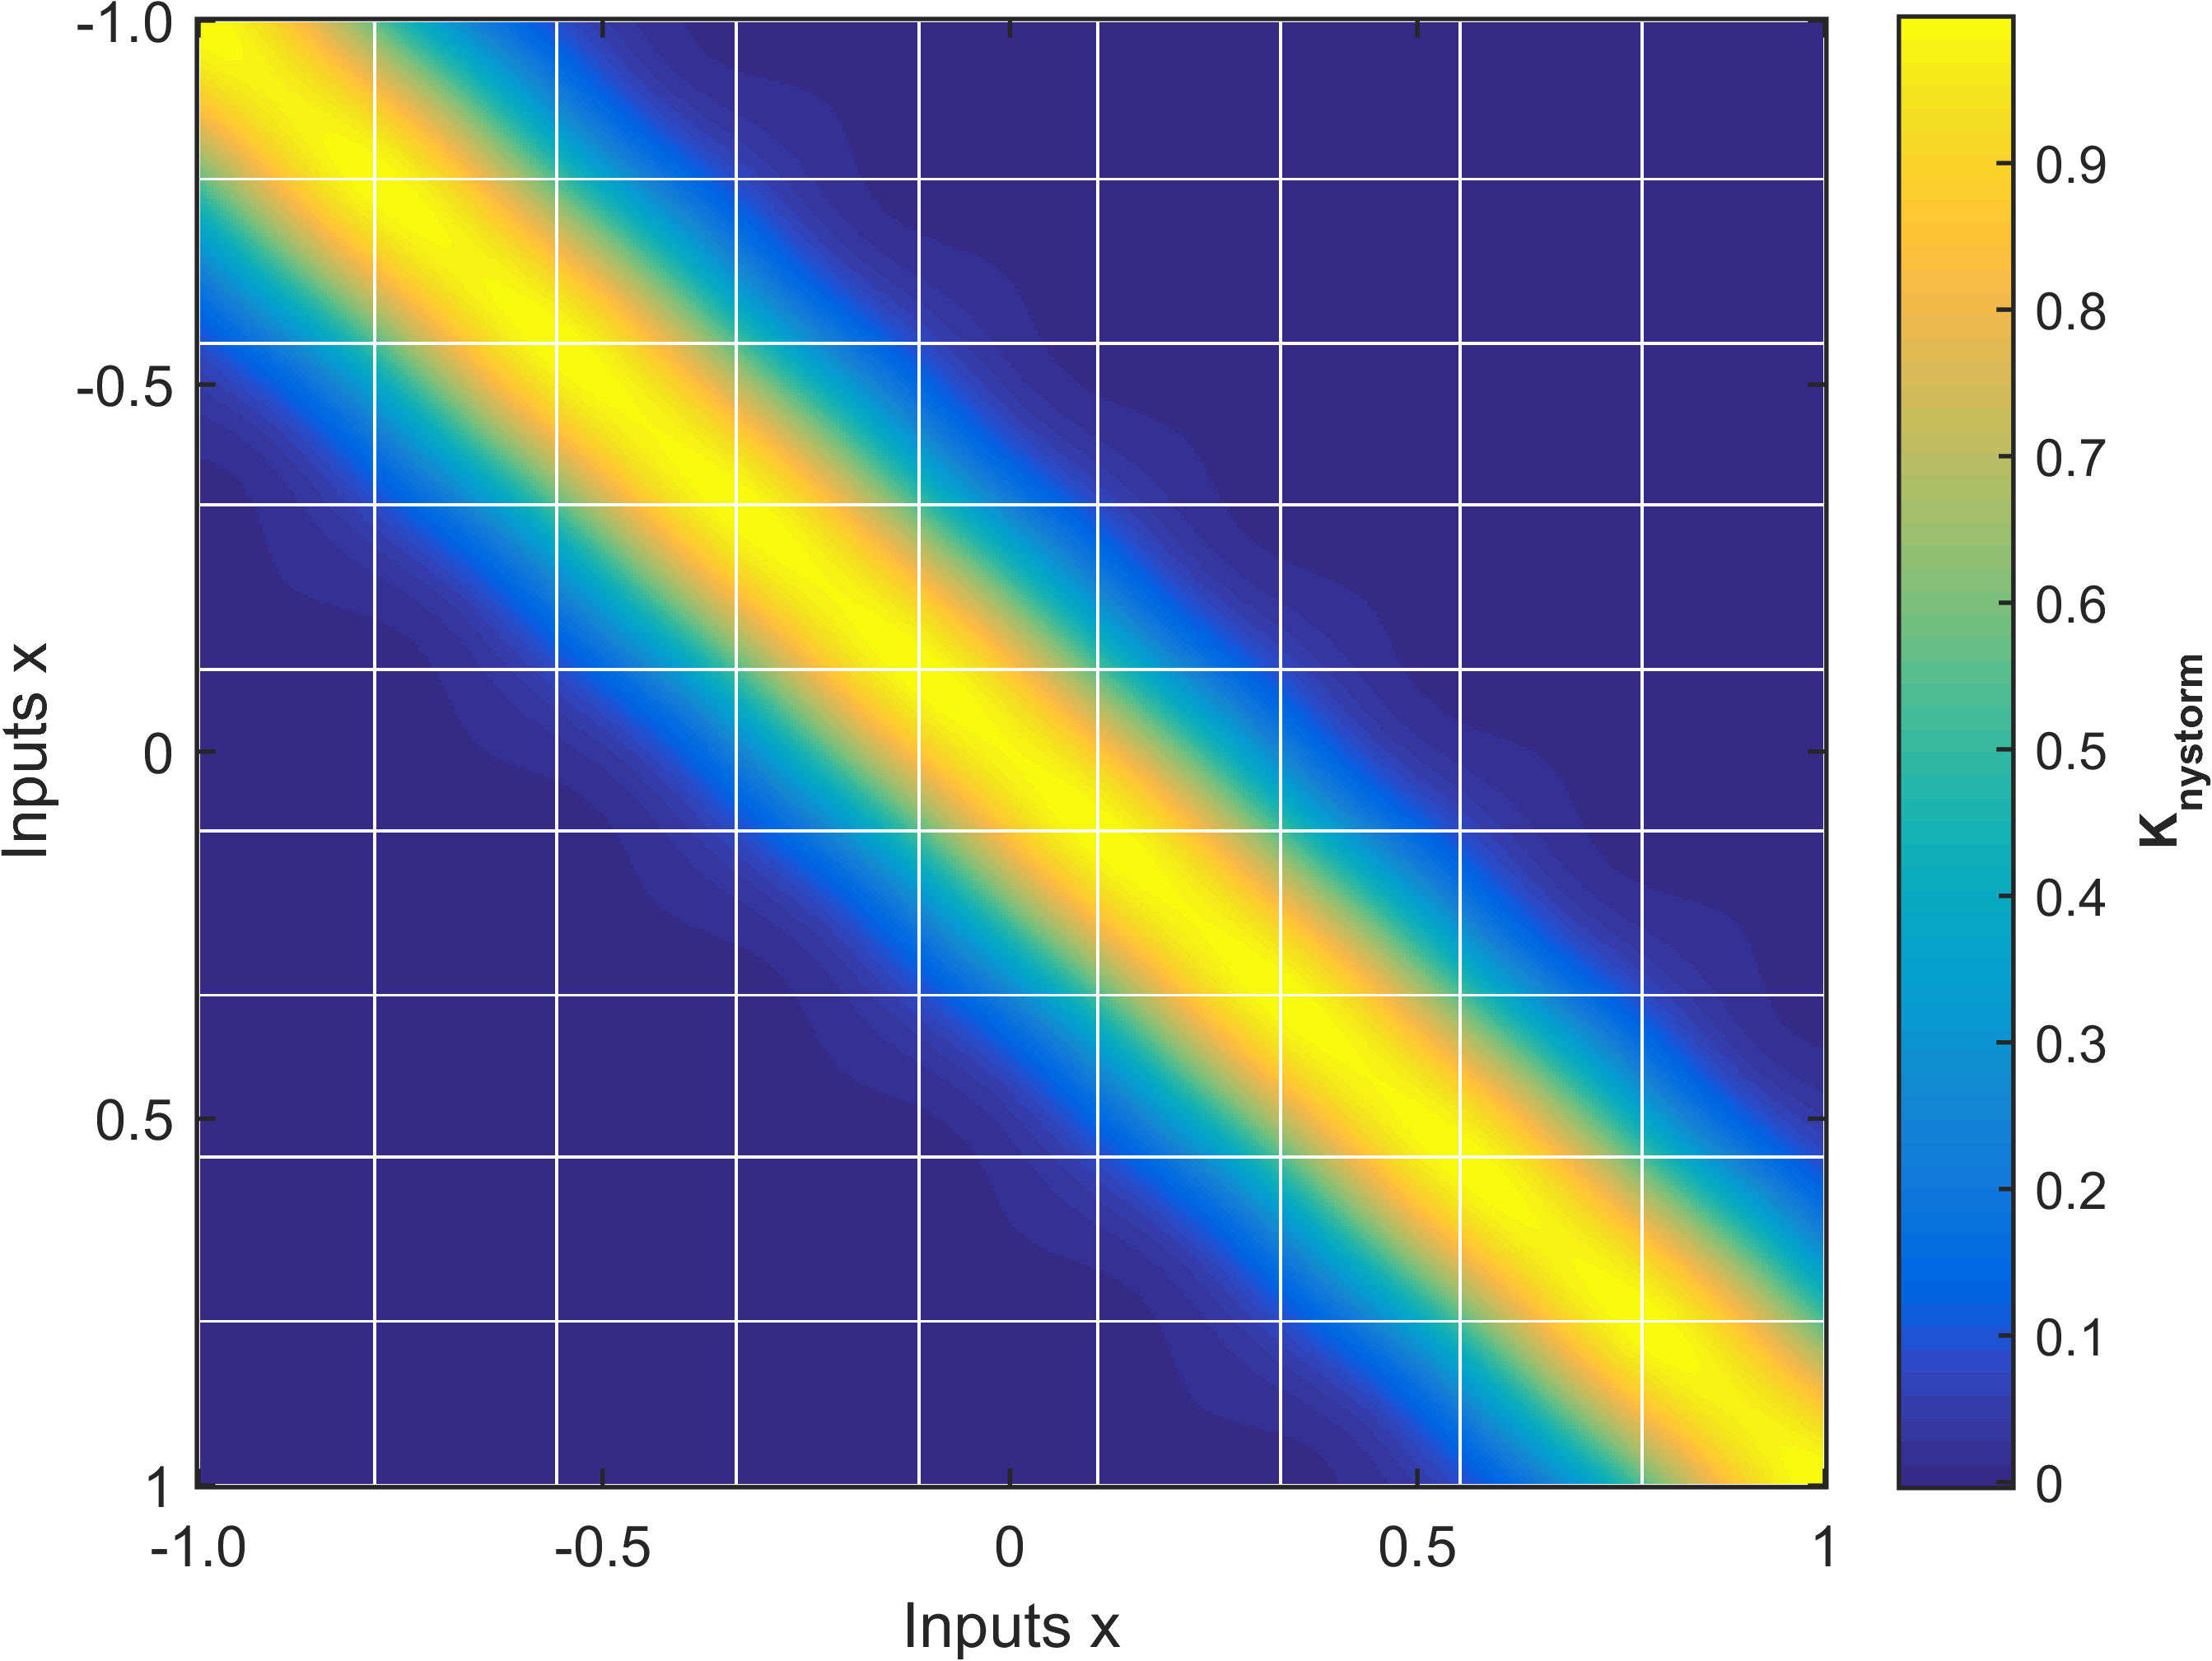
\includegraphics[width=0.45\textwidth]
        {images/part1/nystormSEmatrixUniform}
        \label{subFignystormSEmatrixUniform}
  }\quad
  
       \caption{Approximate Gram matrix for a SE kernel using Nystr\"{o}m approximation.}\label{figGPNystormGramMatrix}
\end{figure}

Later, \cite{Snelson06sparsegaussian} proposed the Fully Independent Training Conditional (FITC) approach which corrects the diagonal terms of the Gram matrix and improves the prediction capabilities (equation \ref{eqnSparseNystormGram}).

\begin{equation}\label{eqnSparseFITCGram}
\myMatrix{K_{FITC}(X, X)} = diag[\myMatrix{K(X, X)} - \myMatrix{K_{Nystorm}(X, X)}] + \myMatrix{K_{Nystorm}(X, X)}
\end{equation}

Note that calculating $diag(\myMatrix{K(X, X)})$ is an $\mathcal{O}\left ( N \right )$ operation and thus does not significantly impact the time taken. 

The posterior distribution for the approximate prior can be derived similarly \cite{williams2001using} and is a Gaussian. The predictive mean, and predictive variance are written as equation \ref{eqNoisyNystormPredictiveMean} and equation \ref{eqNoisyNystormPredictiveCovariance}. Here, $\\myMatrix{K_{Approximate}(X, X')}$ can be the approximated Gram matrix either from the Nystr\"{o}m approximation (equation \ref{eqnSparseNystormGram}) or the FITC approximation (equation \ref{eqnSparseFITCGram}). 
\begin{equation}\label{eqNoisyNystormPredictiveMean}
  \mathbf{E}[f_{approximate}(\VEC{x_{*}})] = \VEC{k_{Xx_{*}}}^{T}( \myMatrix{K_{Approximate}(X, X')} + \sigma^{2}_{n}\myMatrix{I})^{-1} \VEC{y}
  \end{equation}
\begin{equation}\label{eqNoisyNystormPredictiveCovariance}
	Cov[f_{approximate}(\VEC{x_{*}})] = k_{x_{*}x_{*}} - \VEC{k_{Xx_{*}}}^{T}( \myMatrix{K_{Approximate}(X, X')} + \sigma^{2}_{n}\myMatrix{I} )^{-1} \VEC{k_{Xx_{*}}}
  \end{equation}


By approximating the $\myMatrix{K(X, X)}$ using inducing points, we have effectively changed the GP prior. This means that $\myMatrix{X^{m}}$ have also become the hyper-parameters of our GP. Hence we should fine-tune locations of $\myMatrix{X^{m}}$ and the hyper-parameters $\VEC{\theta}$ to obtain a good prediction of our data. The marginal likelihood for the approximate prior (equation \ref{equationApproximateML}) can be written similarly as equation \ref{equationMarginalLikelihood}.

\begin{equation}\label{equationApproximateML}
    \Pr[\VEC{y} \mid \myMatrix{X}, \myMatrix{X^{m}}, \VEC{\theta}] = \mathcal{N}(0 , \myMatrix{K_{Approximate}(X, X')} + \sigma^{2}_{n}\myMatrix{I})
\end{equation}

The approximate marginal likelihood (equation \ref{equationApproximateML}) has more parameters ($\myMatrix{X^{m}}$ and $\VEC{\theta}$) to fine-tune when compared to the old, exact marginal likelihood (equation \ref{eqExactNLML}). Hence, the maximization of the marginal likelihood in equation \ref{equationApproximateML} is prone to over-fitting especially when the number of inducing inputs is large. This means that if we keep on increasing the number of inducing points, a time will come when we will tend to decrease the accuracy of our predictions on the test data set. The variational approximation (detailed next) approach overcomes this issue of over-fitting by adding a regularization term penalizing over-fitting.

\subsection{Variational Approximation}\label{subSecVariationalApprox} 
The variational approximation does not attempt to approximate the Gram matrix. Instead, it assumes a probability distribution $q(f)$ of the true posterior distribution $p(f \mid y)$ and minimizes the distance between the two \cite{Titsias09variationallearning}. 

The $q(f)$ is written in terms of inducing points ($\myMatrix{X^{m}}$) and the KL divergence $KL(q||p)$\footnote{KL divergence is a measure of distance between two probability distributions} is minimized between the variational distribution $q$ and true distribution $p$. When we minimize the KL divergence, we are making the assumed distribution closer to true distribution and hence improving the values of ($\myMatrix{X^{m}}$) and $\VEC{\theta} $. This minimization of KL divergence is equivalently expressed as the maximization of equation \ref{equationLowerBoundVarNLML}

\begin{equation}\label{equationLowerBoundVarNLML}
F_{V} = log(\mathcal{N}[0, \myMatrix{K_{Nystorm}(X, X)} + \sigma_{n}^{2}\myMatrix{I} ]) - \textcolor{blue}{\frac{1}{2\sigma_{n}^{2}}Tr(\myMatrix{K_{XX}} - \myMatrix{K_{Nystorm}(X, X)})}
\end{equation}

Notice the similarity between equation \ref{equationLowerBoundVarNLML} and \ref{equationApproximateML}. The novelty of the above objective function is that it contains a regularization term: $\textcolor{blue}{\frac{1}{2\sigma_{n}^{2}}Tr(\myMatrix{K_{XX}} - \myMatrix{K_{Nystorm}(X, X)})}$. Thus, $F_{V}$ attempts to maximize the marginal likelihood as derived for Nystr\"{o}m approximation and simultaneously minimizes the trace. When the regularization term tends to zero ($\myMatrix{K_{XX}} = \myMatrix{K_{Nystorm}(X, X)}$), it means that the inducing variables can exactly reproduce the true Gram Matrix. 

\sloppy The posterior distribution for variational inference approximation is the same as the one derived for Nystr\"{o}m approximation. The difference between Nystr\"{o}m approximation and variational approximation is the addition of regularization parameter ($\textcolor{blue}{\frac{1}{2\sigma_{n}^{2}}Tr(\myMatrix{K_{XX}} - \myMatrix{K_{Nystorm}(X, X)})}$) while optimizing $\myMatrix{X^{m}}$ and $\VEC{\theta}$, this additional term reduces over-fitting.

\subsection{Experiments}\label{subsecNystromExperiments}
In this section, we conduct experiments on a toy-data set to observe the accuracy of Nystr\"{o}m approximation for varying number and location of inducing points. The basic toolbox used for this section is GPML provided with \cite{Rasmussen2005} on MATLAB 2014b. All experiments were performed on an Intel quad-core processor with 4Gb RAM. 

10-fold Cross Validation (CV) will be used to assess the performance of the prediction. CV is a technique where the dataset is partitioned as the test set and training set. A model is learned using the training set and Root Mean Square Error (RMSE) is calculated between the prediction and test set as a measure of accuracy. In the 10-fold version of CV, the dataset will be randomly partitioned into 10 subsets containing an equal number of points. Of the 10 subsets, a single subset is retained as the test dataset, and the remaining 9 (10 - 1) subsets are used as training data. The cross-validation process is then repeated 10 times (the folds), with each of the k subsets used exactly once as the validation data.

The toy data set ($\mathcal{D}_{3}$) was generated at 1000 input points $\myMatrix{X} = \{[-1:0.002:1]\}$ by sampling a random function from a GP\footnote{$(\Pr[\VEC{y} \mid \myMatrix{X}, \VEC{\theta}, \sigma_{n}] = GP(0, k_{SE}(\myMatrix{x}, \myMatrix{x'}, \theta = [1, 0.1]) + (0.3)^{2}\myMatrix{I})$} with zero mean, SE covariance function ($\VEC{\theta} = [1, 0.1]$) and noise $\sigma_{n} = 0.3$. Code \ref{codeDataset3} generates the dataset $\mathcal{D}_{3}$.

\begin{mdframed}[hidealllines=true,backgroundcolor=lightgray!20]
\lstinputlisting[caption={Code for toy dataset 3}, 
                    captionpos=b, 
                    label={codeDataset3}, 
                    backgroundcolor = \color{MatlabCellColour},
                    style=Matlab-editor,
                    basicstyle=\color{black}\ttfamily\small]
                    {codes/chapter3/generatingDataset3.m}
\end{mdframed}

Figure \ref{predictionOfm10_242} is the prediction of the GP obtained after Nystr\"{o}m approximation using 10 inducing points. The solid black line defines the mean function, blue region defines 95\% confidence interval (2$\sigma$) distance away from the mean. The points denoted by `+' sign are initial locations of inducing points, while the points denoted by `*' sign are locations of inducing points after optimization. The points denoted by `.' are the test points for this fold of the 10-fold CV. 

Notice the inducing points, while initially randomly distributed are later uniformly distributed due to optimization of marginal likelihood. In this case, since the training points are randomly distributed, uniformly distributed inducing inputs are better approximations of the Gram matrix. In cases where training data set tends to be dense in one region and sparse in another region, lesser inducing points get allocated at the dense region and more get allocated at the sparse region. This happens because the information contained in a dense cluster of data-points can be approximated by a fewer data points (points in a neighbourhood are similar (section \ref{subSecCH2Covariance}) \cite{Snelson06sparsegaussian}.

Figure \ref{boxPlotsOfPerformance_242} are 10-fold RMSE box-plots for varying number of inducing points. The box-plots in red are cases when only the hyper-parameters were optimized while inducing inputs were distributed randomly.The box-plots in blue are the cases when both locations of inducing points and hyper-parameters are optimized. The accuracy of prediction improves with increasing number of inducing points. Accuracy is better when both locations of inducing points and hyper-parameters are optimized. Since the noise in the generated toy-data is $\sigma_{n}=0.3$, it is the best achievable RMSE value. Models constructed when optimizing both $\VEC{\theta}, \myMatrix{X^{m}}$ reach this RMSE limit for $M = 20$. After $M=50$, accuracy is similar for both the optimization routines. As a thumb rule, if $M = \frac{N}{10}$, then randomly distributing the inducing points and optimizing $\VEC{\theta}$ will be sufficient to give a good prediction \cite{cao2013efficient}, while if $M = \frac{N}{50}$ then both inducing points and hyper-parameters should be optimized. 

\begin{figure}[!ht]
  \centering
    \subfigure[{Posterior between a Nystr\"{o}m approximated SE prior with 10 inducing inputs and training data. The solid black line defines the mean function, blue region defines 95\% confidence interval (2$\sigma$) distance away from the mean. The points denoted by `+' sign are initial locations of inducing points, while the points denoted by `*' sign are locations of inducing points after optimization.}]
  {
        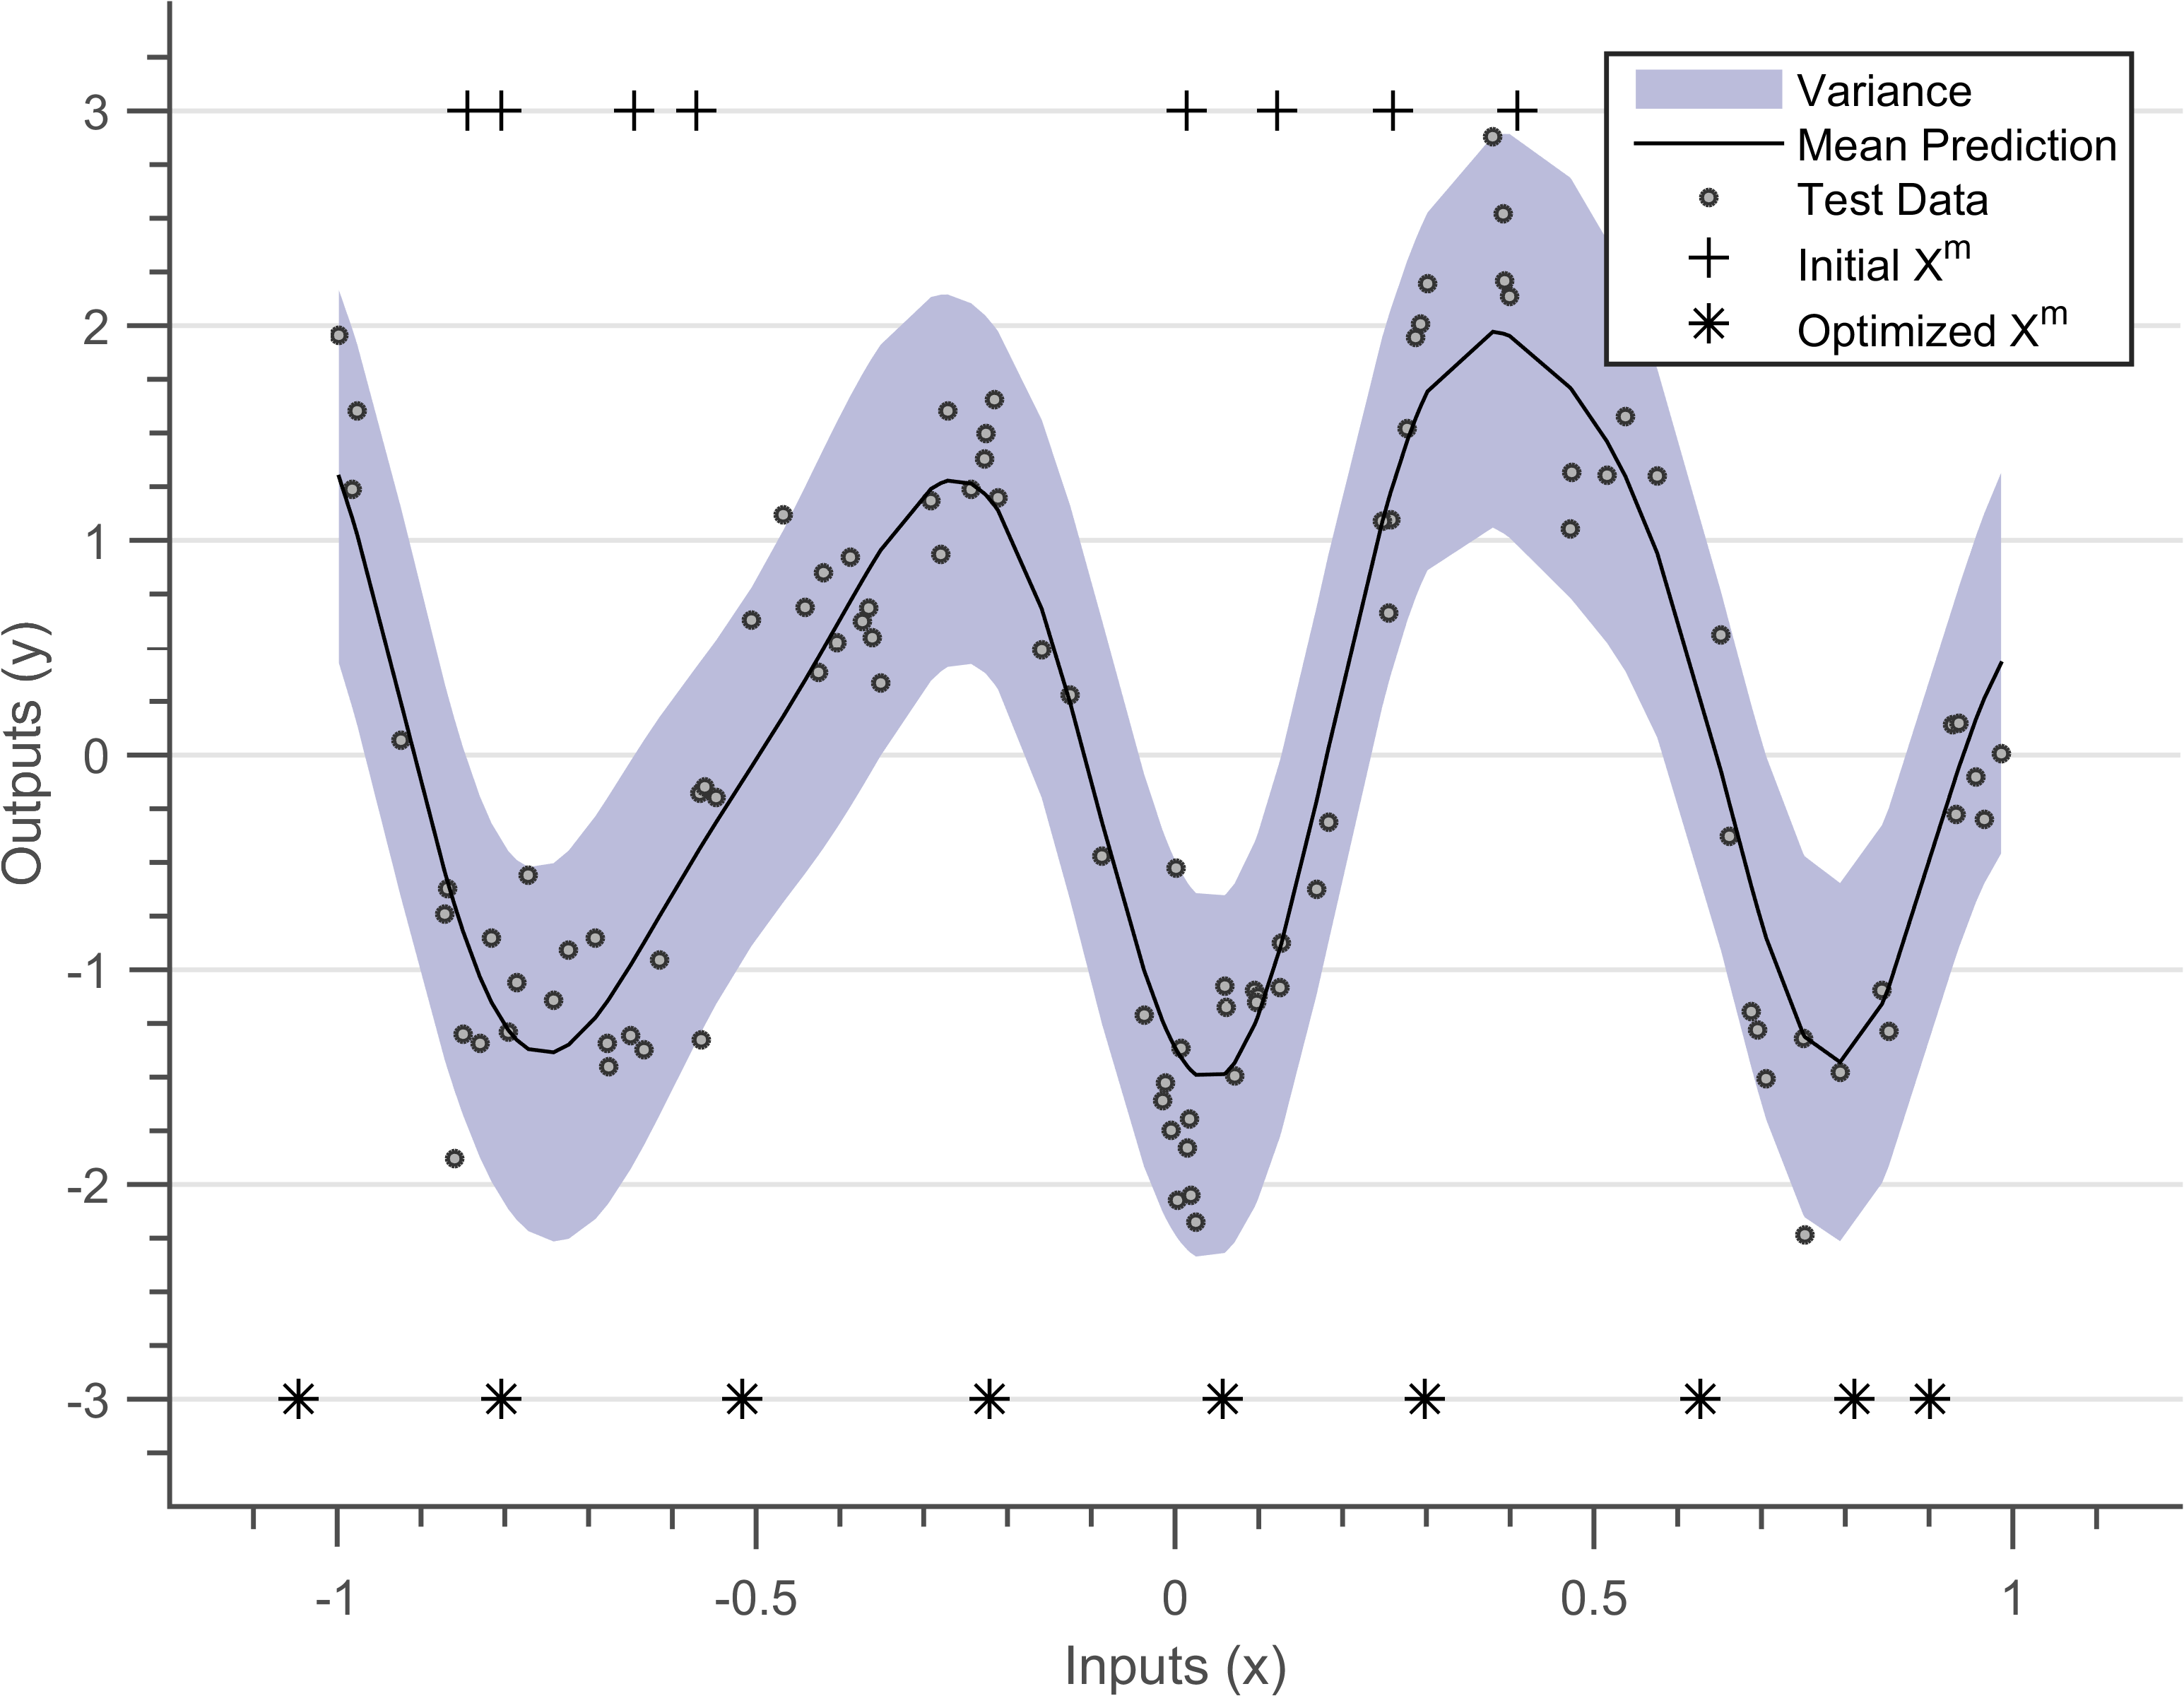
\includegraphics[width=0.45\textwidth]
        {images/part1/predictionOfm10_242}
        \label{predictionOfm10_242}
  }\quad
\subfigure[{10-fold RMSE box-plots for varying number of inducing points. The box-plots in red are cases when only the hyper-parameters $\VEC{\theta}$ were optimized while inducing inputs were distributed randomly. The box-plots in blue are the cases when both locations of inducing points $X^{m}$ and hyper-parameters $\VEC{\theta}$ are optimized. }]
  {
        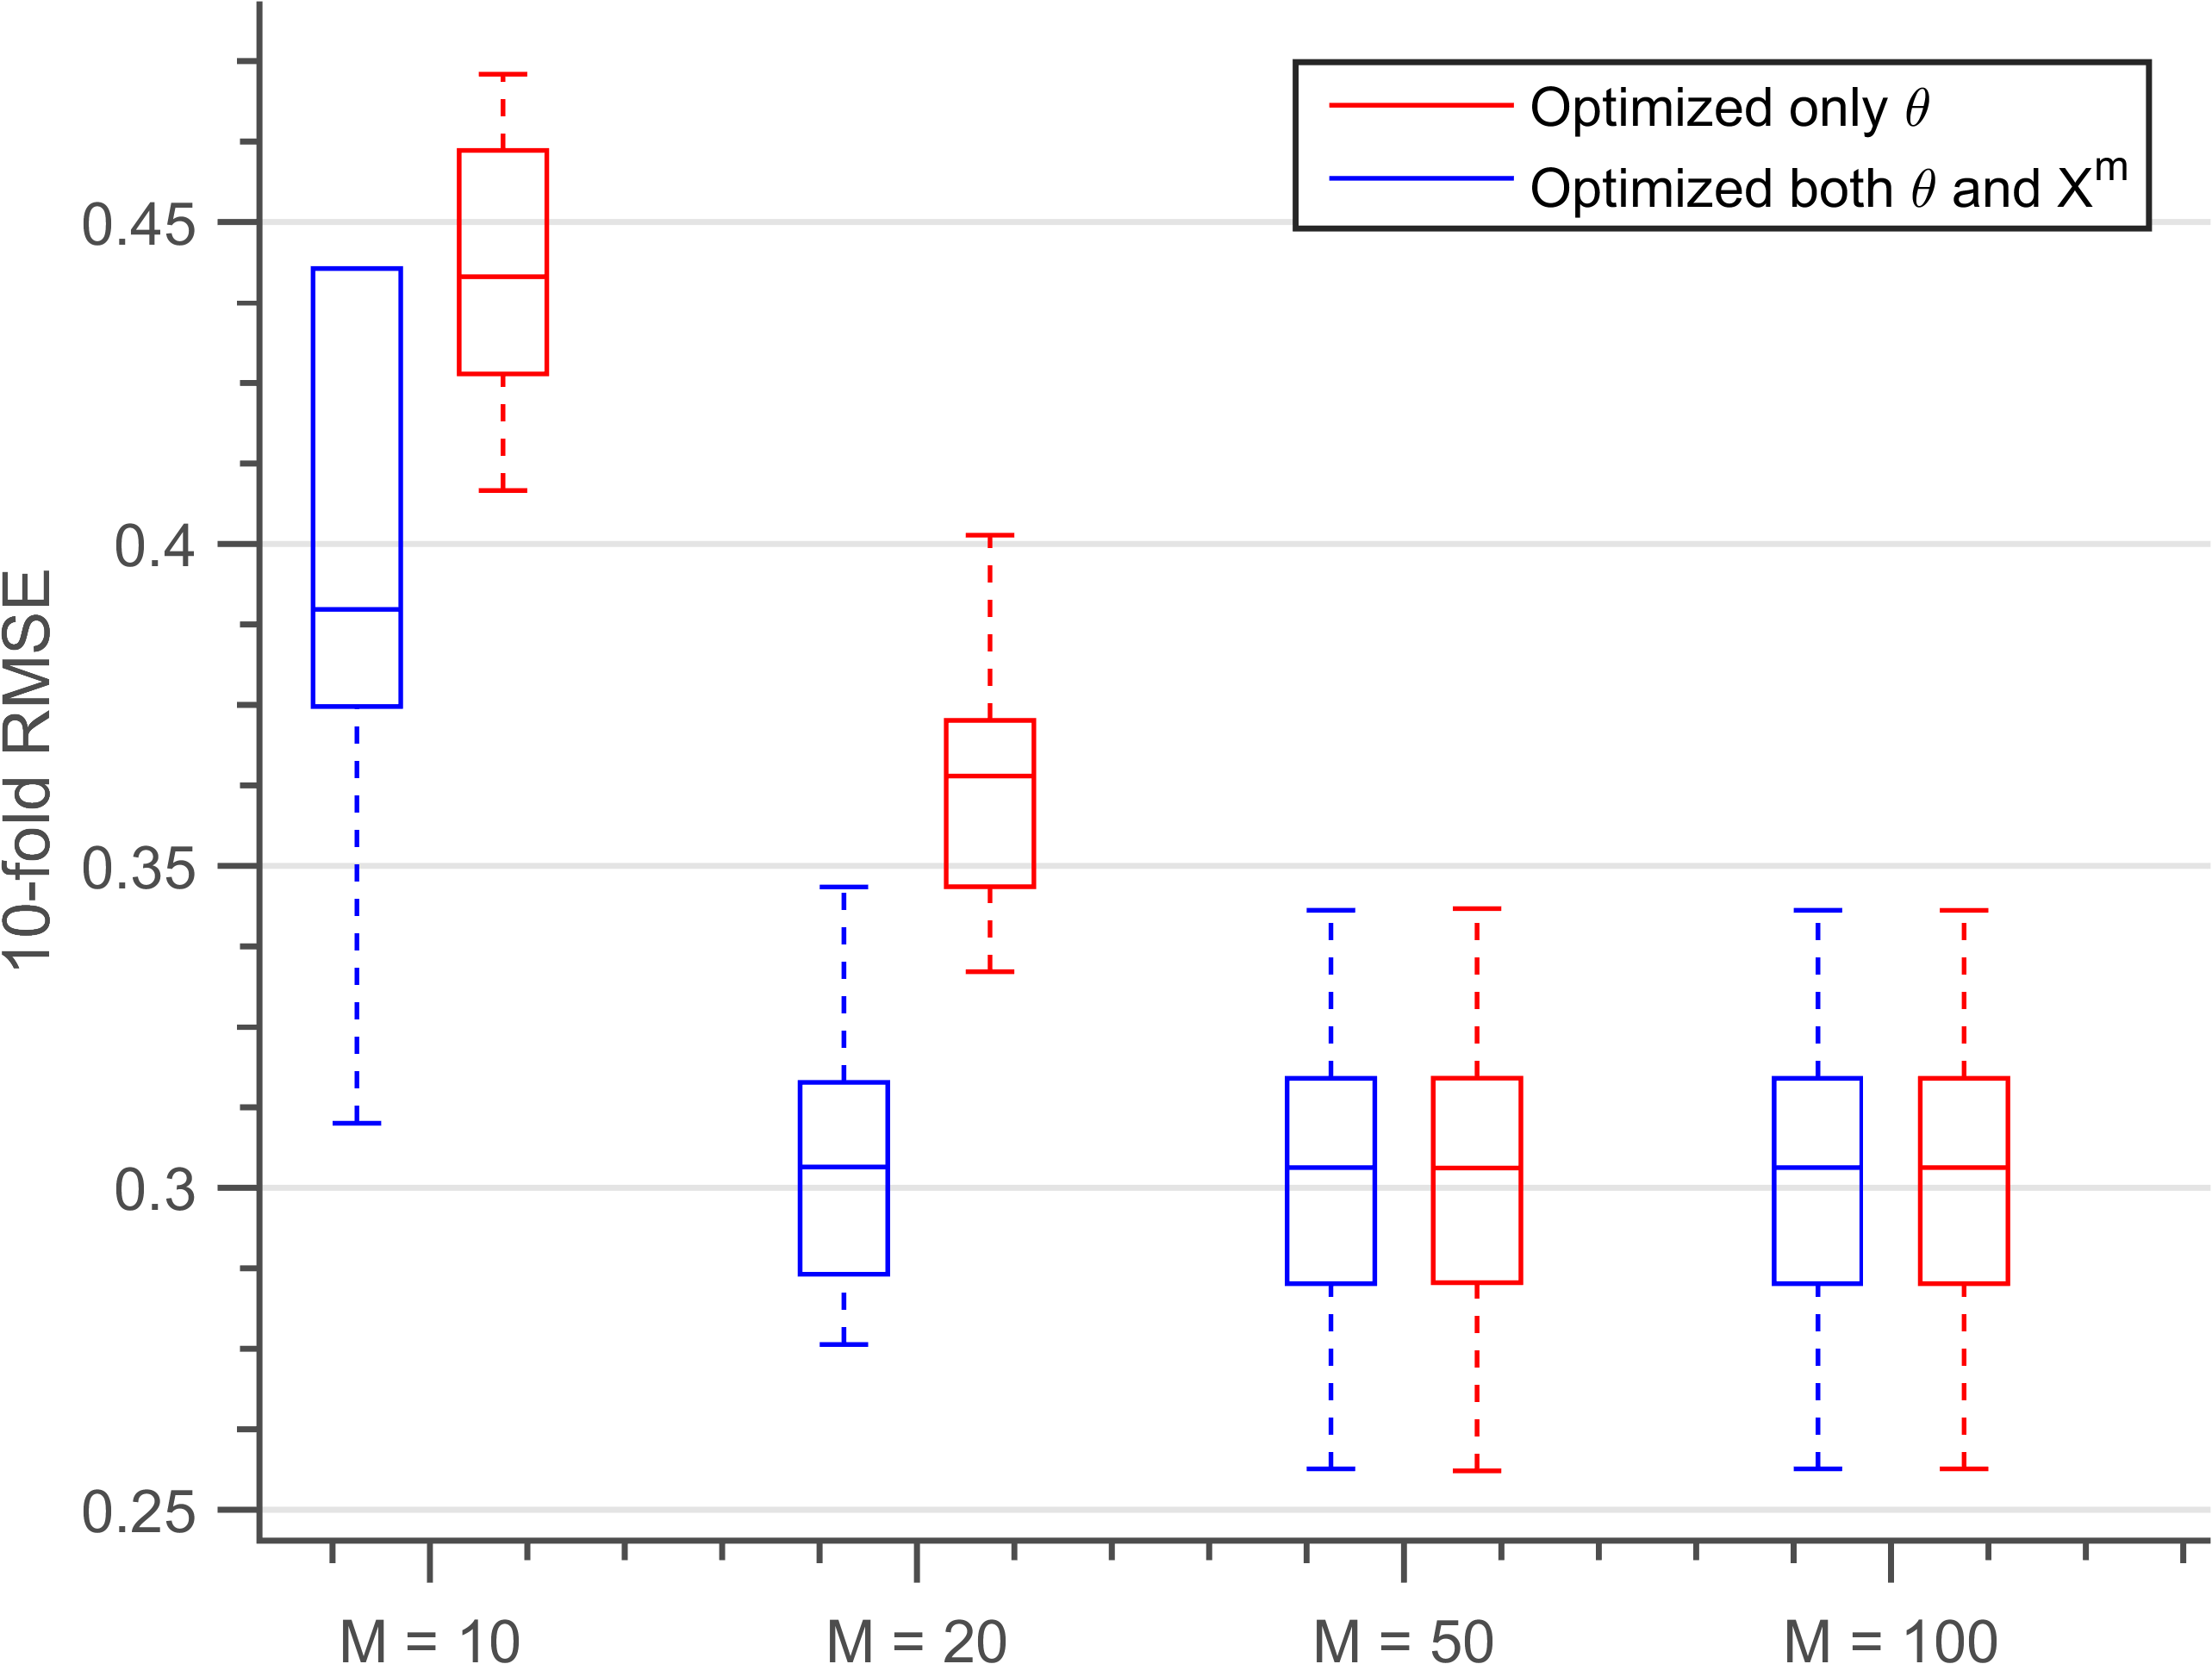
\includegraphics[width=0.45\textwidth]
        {images/part1/boxPlotsOfPerformance_242}
        \label{boxPlotsOfPerformance_242}
  }\quad
  
       \caption{Results of Nystr\"{o}m Approximation on a toy-data set of size $N=1000$ }\label{figGPPredictionNystorm}
\end{figure}

Global low-rank approximations are best suited for the case of spread out Gram matrices (example high length-scale SE priors). We have seen three types of low-rank approximation algorithms in this section. While Nystr\"{o}m and FITC approximations are the simplest method to approximate Gram matrix, finding optimal locations of the inducing points can often lead to over-fitting. We then look at variational approximation procedure which adds a regularization term while finding inducing points, thereby, penalizing over-fitting. The lower computational cost due to sparse approximations, scales sparse GPs to the training set of sizes $N \sim \mathcal{O}(5 \times 10^5)$. \cite{Gal2014Distributed} propose a distributed architecture for scaling variational sparse GPs. In the next section we look at how to approximate Gram matrices using mixture of experts, this enables us to massively scale GPs to sizes $N > \mathcal{O}(10^6)$ by exploiting distributed architecture.

\section{Distributed Gaussian Process}\label{secDgp}
In the year 2006 Netflix organized a machine learning competition, to create a recommendation algorithm for its users. Teams from all over the world competed in this competition to make the best video recommendation algorithm. As the competition progressed, teams started figuring out that the accuracy increases upon combining algorithms developed by multiple teams. The winner and the runner-up were model ensembles of hundreds of algorithms. Creating model ensembles (also called mixture of experts) is now a standard practice in many learning competitions \cite{bauer1998empirical}. 

Mixture of experts in GPs use bagging, where subsets of data are generated, individual GPs are trained on these subsets, and their results are finally combined \cite{chen2009bagging}. If the data set is partitioned  into $N_{experts}$ subsets, such as $\mathcal{D}^{(i)} = {\myMatrix{X^{(i)}}, \VEC{y^{(i)}}}, i \in 1, \ldots N_{experts}$. Then each subset of data $\mathcal{D}^{(i)}$ learns an individual GP model, which are to be combined together to give the final predictions . Due to this independent learning, choosing hyper-parameters, and calculating predictions become easily parallelizable and indifferent to the computational infrastructure. 

\sloppy Initially, these model types were used to highlight local features in the data \cite{rasmussen2002infinite}. Later,  \cite{ng2014hierarchical} proposed to use the parallel feature to speed up predictions. Instead of learning a different GP for each subset, we tie all the different experts using one single set of hyperparameters. This is equivalent to assuming one single GP for the whole data-set, thus the experts are same but they each have access to different dataset. This tying of experts greatly reduces the number of hyper-parameters, acts as a regularization, and inhibits over-fitting. Equation \ref{distributedGPPrior} denotes an independent GP prior for each expert $\mathcal{D}^{(i)}$ such that the hyper-parameters $\VEC{\theta}$ and $\sigma_{n}$ are same for all experts.

\begin{equation}\label{distributedGPPrior}
    \Pr[\VEC{y^{(i)}} \mid \myMatrix{X^{(i)}}, \VEC{\theta}, \sigma_{n}] = GP(0, \myMatrix{K(\VEC{X^{(i)}}, X^{(i)'}, \theta)} + \sigma^{2}_{n}\myMatrix{I}) 
\end{equation}

The sample code \ref{codeClusteringIntoExperts} presents a method to randomly clusterize dataset across $6$ experts.
\begin{mdframed}[hidealllines=true,backgroundcolor=lightgray!20]
\lstinputlisting[caption={Randomly clustering points into experts}, 
                    captionpos=b, 
                    label={codeClusteringIntoExperts}, 
                    backgroundcolor = \color{MatlabCellColour},
                    style=Matlab-editor,
                    basicstyle=\color{black}\ttfamily\small]
                    {codes/chapter3/clusteringPointsInExperts.m}
\end{mdframed}

Figure \ref{subFigdistributedKernelRandomExperts} is an approximate Gram matrix using the above approximation, for a SE Kernel with $(\VEC{\theta} = [1, 0.2])$ at the input points $\myMatrix{X^{*}} = \{[0:0.02:1]\}$. 5 experts each having 100 points are chosen, points in the experts are distributed randomly, this gives the approximate Gram matrix the scattered shape. Figure \ref{subFigDistributedKernel} is an approximate Gram matrix using same approximation, and uniformly distributed experts. 5 experts each having 100 points are chosen, The first expert has first set of 100 points, the second expert has the second set of 100 points and so on. Both the figures are trying to approximate the Gram matrix of the matrix in figure \ref{subFigcovSEmatrix_1}. The Gram matrix with randomly chosen experts has a more global nature but lacks many high variance regions. The Gram matrix for uniformly chosen experts retains more local features. Inversion of this Gram matrix is an operation of complexity $\mathcal{O}(N_{experts}P^{3})$, where $P$ is the number of points in an expert.

\begin{figure}[!ht]
  \centering
    \subfigure[{Approximated Gram matrix using distributed GP approximation for a SE Kernel with $(\VEC{\theta} = [1, 0.2])$ (figure \ref{subFigcovSEmatrix_1}) at the input points $\myMatrix{X^{*}} = \{[0:0.02:1]\}$. Points in the experts are distributed randomly, this gives the approximate Gram matrix scattered shape.}]
  {
        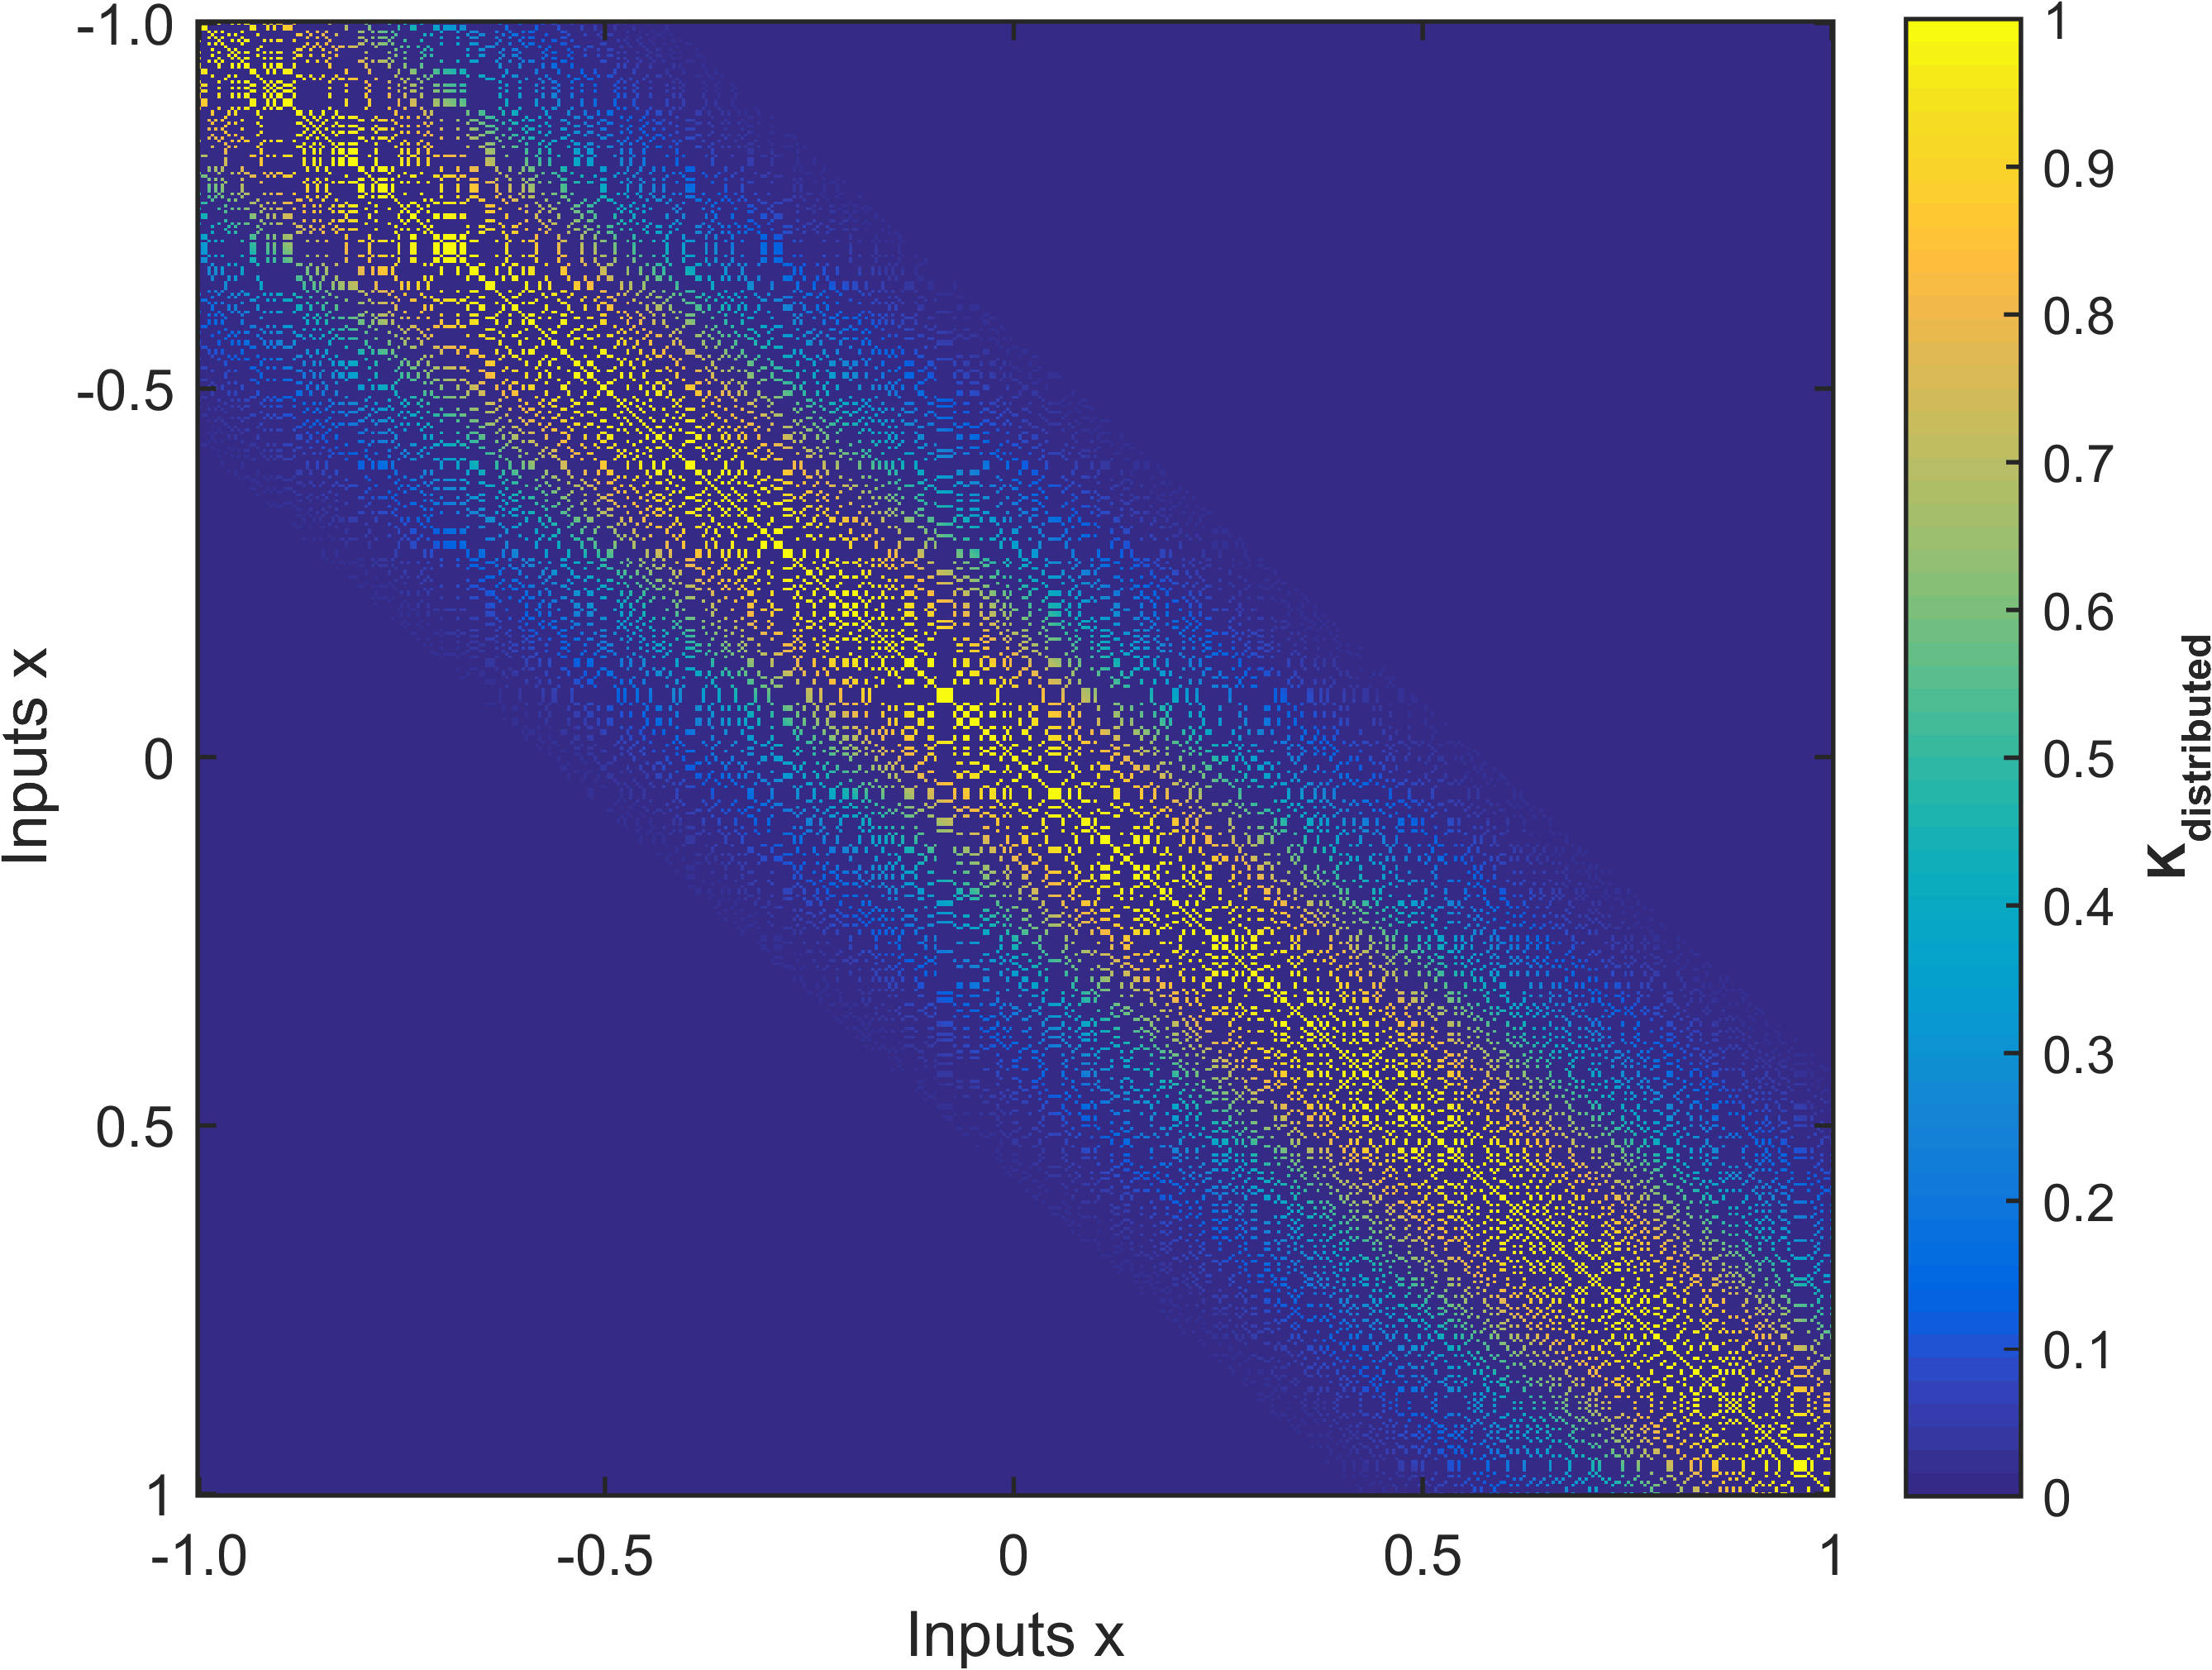
\includegraphics[width=0.45\textwidth]
        {images/part1/distributedKernelRandomExperts}
        \label{subFigdistributedKernelRandomExperts}
  }\quad
\subfigure[{Approximated Gram matrix using distributed GP approximation for a SE Kernel with $(\VEC{\theta} = [1, 0.2])$ (figure \ref{subFigcovSEmatrix_1}) at the input points $\myMatrix{X^{*}} = \{[0:0.02:1]\}$. Points in the experts are distributed uniformly. We can observe that covariance across experts goes to zero.}]
  {
        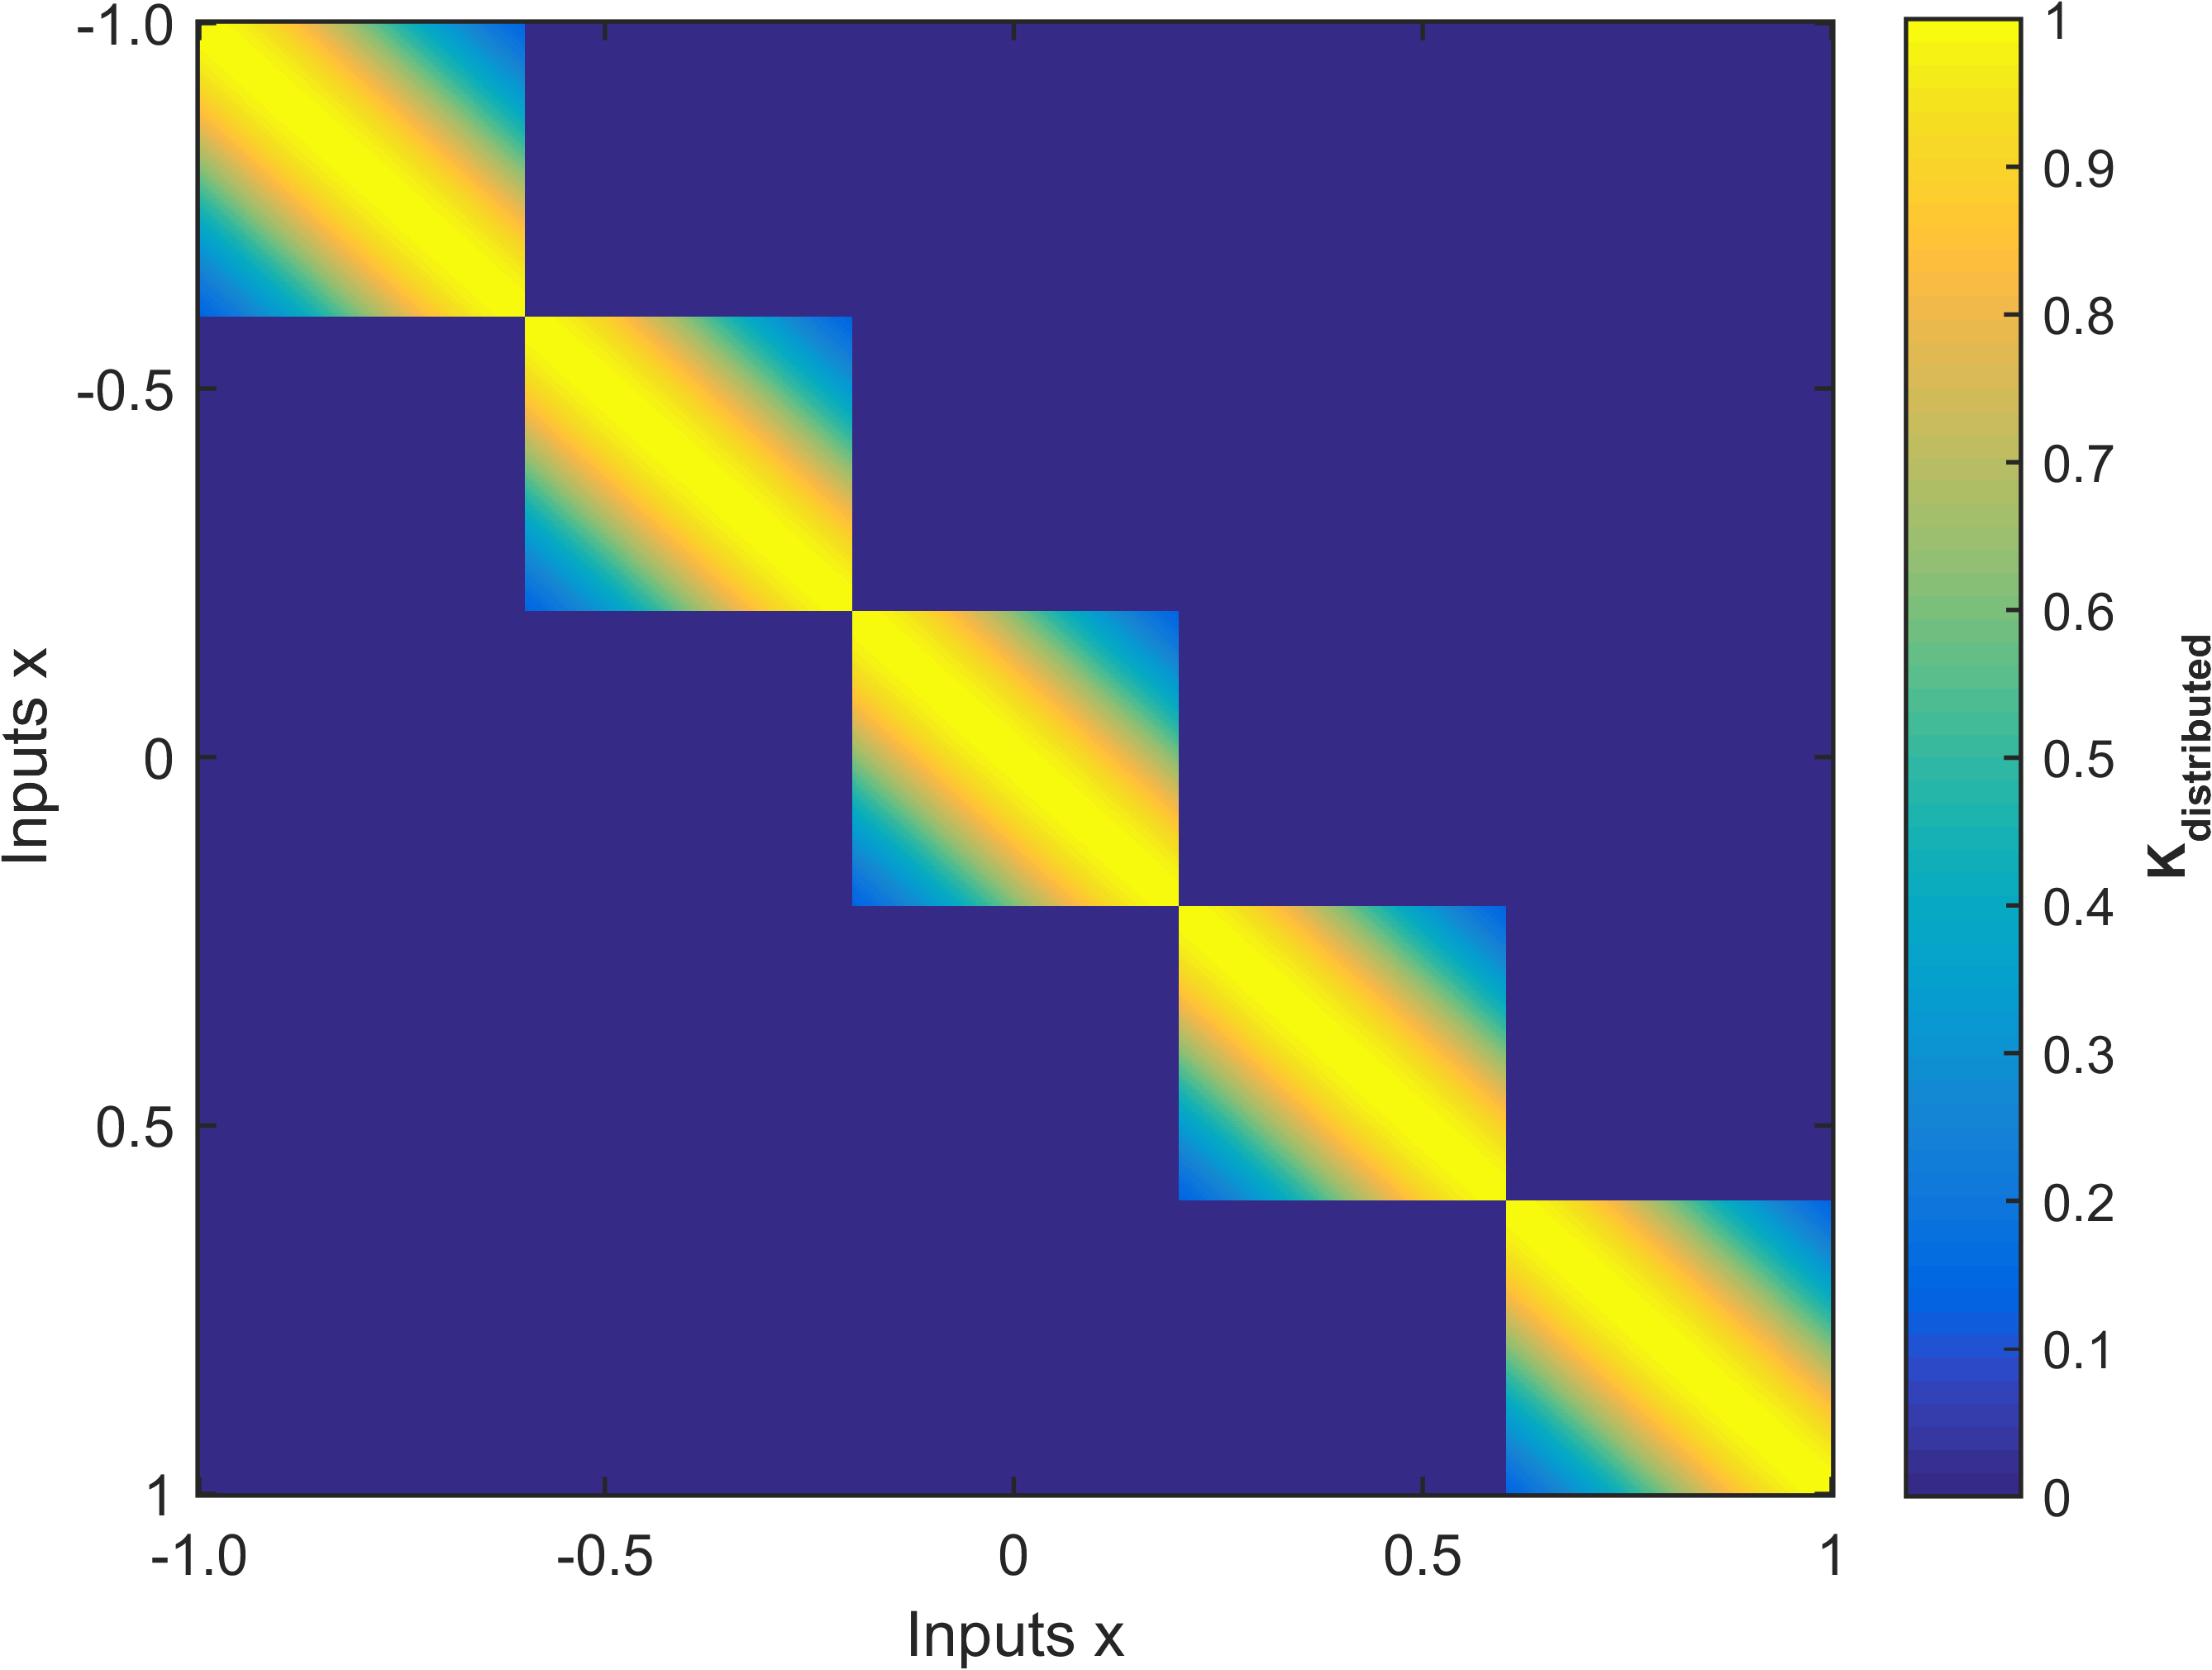
\includegraphics[width=0.45\textwidth]
        {images/part1/distributedKernel}
        \label{subFigDistributedKernel}
  }\quad
  
       \caption{Approximate Gram matrix for a SE kernel using mixture of experts.}\label{figGPApproximateDGPMatrix}
\end{figure}

Since the experts are independent of each other, we can construct a posterior distribution for each expert (equations \ref{eqPredictiveMeanIndividualExpert} and \ref{eqPredictiveCovarianceIndividualExpert}). In the following equations $m^{(i)}(\VEC{x_{*}})$ and $\sigma^{(i)}(\VEC{x_{*}})$ are the mean and covariance predictions from expert $i$ at point $\VEC{x_{*}}$.  

\begin{equation}\label{eqPredictiveMeanIndividualExpert}
  m^{(i)}(y(\VEC{x_{*}})) = \VEC{k_{X^{(i)}x_{*}}}^{T}( \myMatrix{K_{X^{(i)}, X^{(i)'}}} + \sigma^{2}_{n}\myMatrix{I})^{-1} \VEC{y^{(i)}}
  \end{equation}
\begin{equation}\label{eqPredictiveCovarianceIndividualExpert}
	\sigma^{(i)}(y(\VEC{x_{*}})) = k_{x_{*}x_{*}} - \VEC{k_{X^{(i)}x_{*}}}^{T}( \myMatrix{K_{X^{(i)}, X^{(i)'}}} + \sigma^{2}_{n}\myMatrix{I} )^{-1} \VEC{k_{X^{(i)}x_{*}}}
  \end{equation}

\subsection{Combining experts}\label{subSecCombiningExperts}
There are several methods in the literature, which combine the posterior predictions of individual experts, and give a global estimate. The Product of Experts model, uses the independence assumption between experts, and multiplies the individual posterior distribution\footnote{$\Pr[y(\VEC{x_{*}}) \mid \VEC{x_{*}}, \mathcal{D}, \VEC{\theta}] \propto \prod \Pr[\VEC{y^{(i)}} \mid \myMatrix{X^{(i)}}, \mathcal{D}^{(i)}, \VEC{\theta}]$}, but these predictions tend to be overconfident. Another method called the generalized Product of Experts (gPOE), assigns a participation factor to each expert, this is based on the amount of uncertainty in prediction (more confident experts have higher say in prediction)\cite{caoF14}. The Bayesian Committee Machine (BCM) imposes the independence assumption between each expert pair using Bayes Rule, but can result in bad predictions when leaving data regime \cite{tresp2000bayesian}. 

This thesis will use robust Bayesian Committee Machine (rBCM) model to combine the posterior distributions of experts \cite{deisenroth2015distributed}. The rBCM model is an aggregation of all the above three mentioned methods, it combines the confidence weighting parameter of gPOE, with the Bayesian formulation in BCM technique, to generate the following posterior distributions.

\begin{equation}\label{eqMeanDGP}
    m(y(\VEC{x_{*}})) = (Cov(y(\VEC{x_{*}})))^{-2}\sum_{i} \beta_{i}(\sigma^{(i)})^{-2}m^{(i)}(\VEC{x_{*}})
\end{equation}
\begin{equation}\label{eqCovarianceDGP}
    Cov(y(\VEC{x_{*}}))^{^-2} = \sum_{i} \beta_{i}\sigma^{(i)}(y(\VEC{x_{*}})) + (1- \sum_{i} \beta_{i})(k_{x_{*}x_{*}})^{-2}
\end{equation}


$K_{x_{*}x_{*}}$ is the auto-covariance of the prior at prediction point $\VEC{x_{*}}$. $\beta_{k}$ determines the influence of experts on the final predictions \cite{caoF14} and is given as $\beta_{i} = \frac{1}{2}(\log k_{x_{*}x_{*}}^{2} - \log(\sigma^{(i)}(y(\VEC{x_{*}})))^{2})$. Experts which are very confident in their predictions at $\VEC{x_{*}}$ will tend to have low $\sigma^{(i)}$ thereby leading to a higher influence factor $\beta_{i}$.

Due to the independence assumption, the marginal likelihood can be written as a sum of individual likelihoods and then can be optimized to find the best-fit hyperparameters. By approximating the $\myMatrix{K(X, X)}$ in terms of $\mathcal{D}^{(i)}$ and $N_{experts}$ we have again changed the GP prior. This means that the number of experts $N_{experts}$ and clustering of points also impact the prediction capabilities of GP. The below equation \ref{eqDGPNLML} describes the formulation for marginal likelihood. 

\begin{align}\label{eqDGPNLML}
    \log \Pr[\VEC{y} \mid \myMatrix{X}, \mathcal{D}, \VEC{\theta}] \approx \sum_{k=1}^{N_{experts}} \log \Pr[\VEC{y^{(i)}}\mid \myMatrix{X^{(i)}}, \VEC{\theta}]
 \end{align}

The sample code \ref{codelmdDGP} defines the function `logMarginalLikelihoodDGP' which calculates the new log marginal likelihood (equation \ref{eqDGPNLML}) using the experts as defined in code \ref{codeClusteringIntoExperts}. The optimal hyper-parameters can be obtained after maximizing this function with respect to hyper-parameters. 

\begin{mdframed}[hidealllines=true,backgroundcolor=lightgray!20]
\lstinputlisting[caption={log Marginal Likelihood for Distributed GP}, 
                    captionpos=b, 
                    label={codelmdDGP}, 
                    backgroundcolor = \color{MatlabCellColour},
                    style=Matlab-editor,
                    basicstyle=\color{black}\ttfamily\small]
                    {codes/chapter3/logMarginalLikelihoodDGP.m}
\end{mdframed}

Maximizing the above log-marginal likelihood will give the optimal values of hyper-parameters. Points in the experts can be distributed either randomly, or using a clustering scheme (eg. k-means clustering\footnote{k-means algorithm clusters close by points in one cluster. The notion of closeness is defined by some measure of distance}) for stationary kernels k-means clustering should be preferred. The k-means algorithm clusters points based on a measure of distance, points in separate clusters are far away from each other when compared to points in the same cluster. This means that the covariance (for stationary kernels) between separate clusters is significantly lower when compared to points in same cluster. Hence, the cross-covariance across separate clusters can be more easily assumed to be zero.

\subsection{Experiments}\label{subSecDistributedExperiments}
We again conduct experiments on a toy-data set, this time to observe the accuracy of the distributed GP approximation for a varying number of experts. 

Again the 10-fold Cross Validation (CV) will be used to assess the performance of the prediction. The same toy-data set as used in section \ref{subsecNystromExperiments} was used to perform the experiments in this section (1000 data-points from $\Pr[\VEC{y} \mid \myMatrix{X}, \VEC{\theta}, \sigma_{n}] = GP(0, \myMatrix{K_{SE}(X, X', \theta = [1, 0.1])} + (0.3)^{2}\myMatrix{I})$.

Figure \ref{predictionOfm10_243} is the prediction of the GP obtained after distributed approximation using 9 experts and k-means clustering. The solid black line defines the mean function, blue region defines 95\% confidence interval (2$\sigma$) distance away from the mean. The colored points in the points denoted by `*' at the bottom show how different points are distributed across experts, similar colored points belong to one expert. The data denoted by `.' is the test data for one fold of the 10-fold CV. 

The points across experts are uniformly distributed, as can be observed by the coloring scheme. Since the training points are almost uniformly distributed, the k-means algorithm will cluster the points uniformly. The training and the test dataset for figures \ref{predictionOfm10_243} and \ref{predictionOfm10_242} are kept intentionally same. We can thus compare the interpolating properties of both inducing inputs approximation (figure \ref{predictionOfm10_243}) and distributed GP (figure \ref{predictionOfm10_242}). The Nystr\"{o}m approximation has a global smooth shape while the distributed GP approximation retains the local features of the data set. 

Figure \ref{boxPlotsOfPerformance_243} are 10-fold RMSE box-plots for different values of $P$. The box-plots in red are cases when the points are distributed using k-means clustering. The box-plots in blue are the cases when points are distributed randomly. The accuracy of prediction improves with increasing number of points in an expert. Note, the noise in the generated toy-data is $\sigma_{n}=0.3$, it is the best achievable RMSE value. Accuracy is slightly better when experts are distributed using k-means clustering, both being very close to the $0.3$ RMSE limit. As a thumb-rule, setting $P = N/100$, and optimizing the hyper-parameters ($\VEC{\theta}$) is a good enough approximation. 


\begin{figure}[!ht]
  \centering
    \subfigure[{Prediction of the GP obtained after distributed approximation using 9 experts and k-means clustering. The solid black line defines the mean function, blue region defines 95\% confidence interval (2$\sigma$) distance away from the mean. The colored points in the points denoted by `*' at the bottom show how different points are distributed across experts, similar colored points belong to one expert. The data denoted by `.' is the test data for one fold of the 10-fold CV. }]
  {
        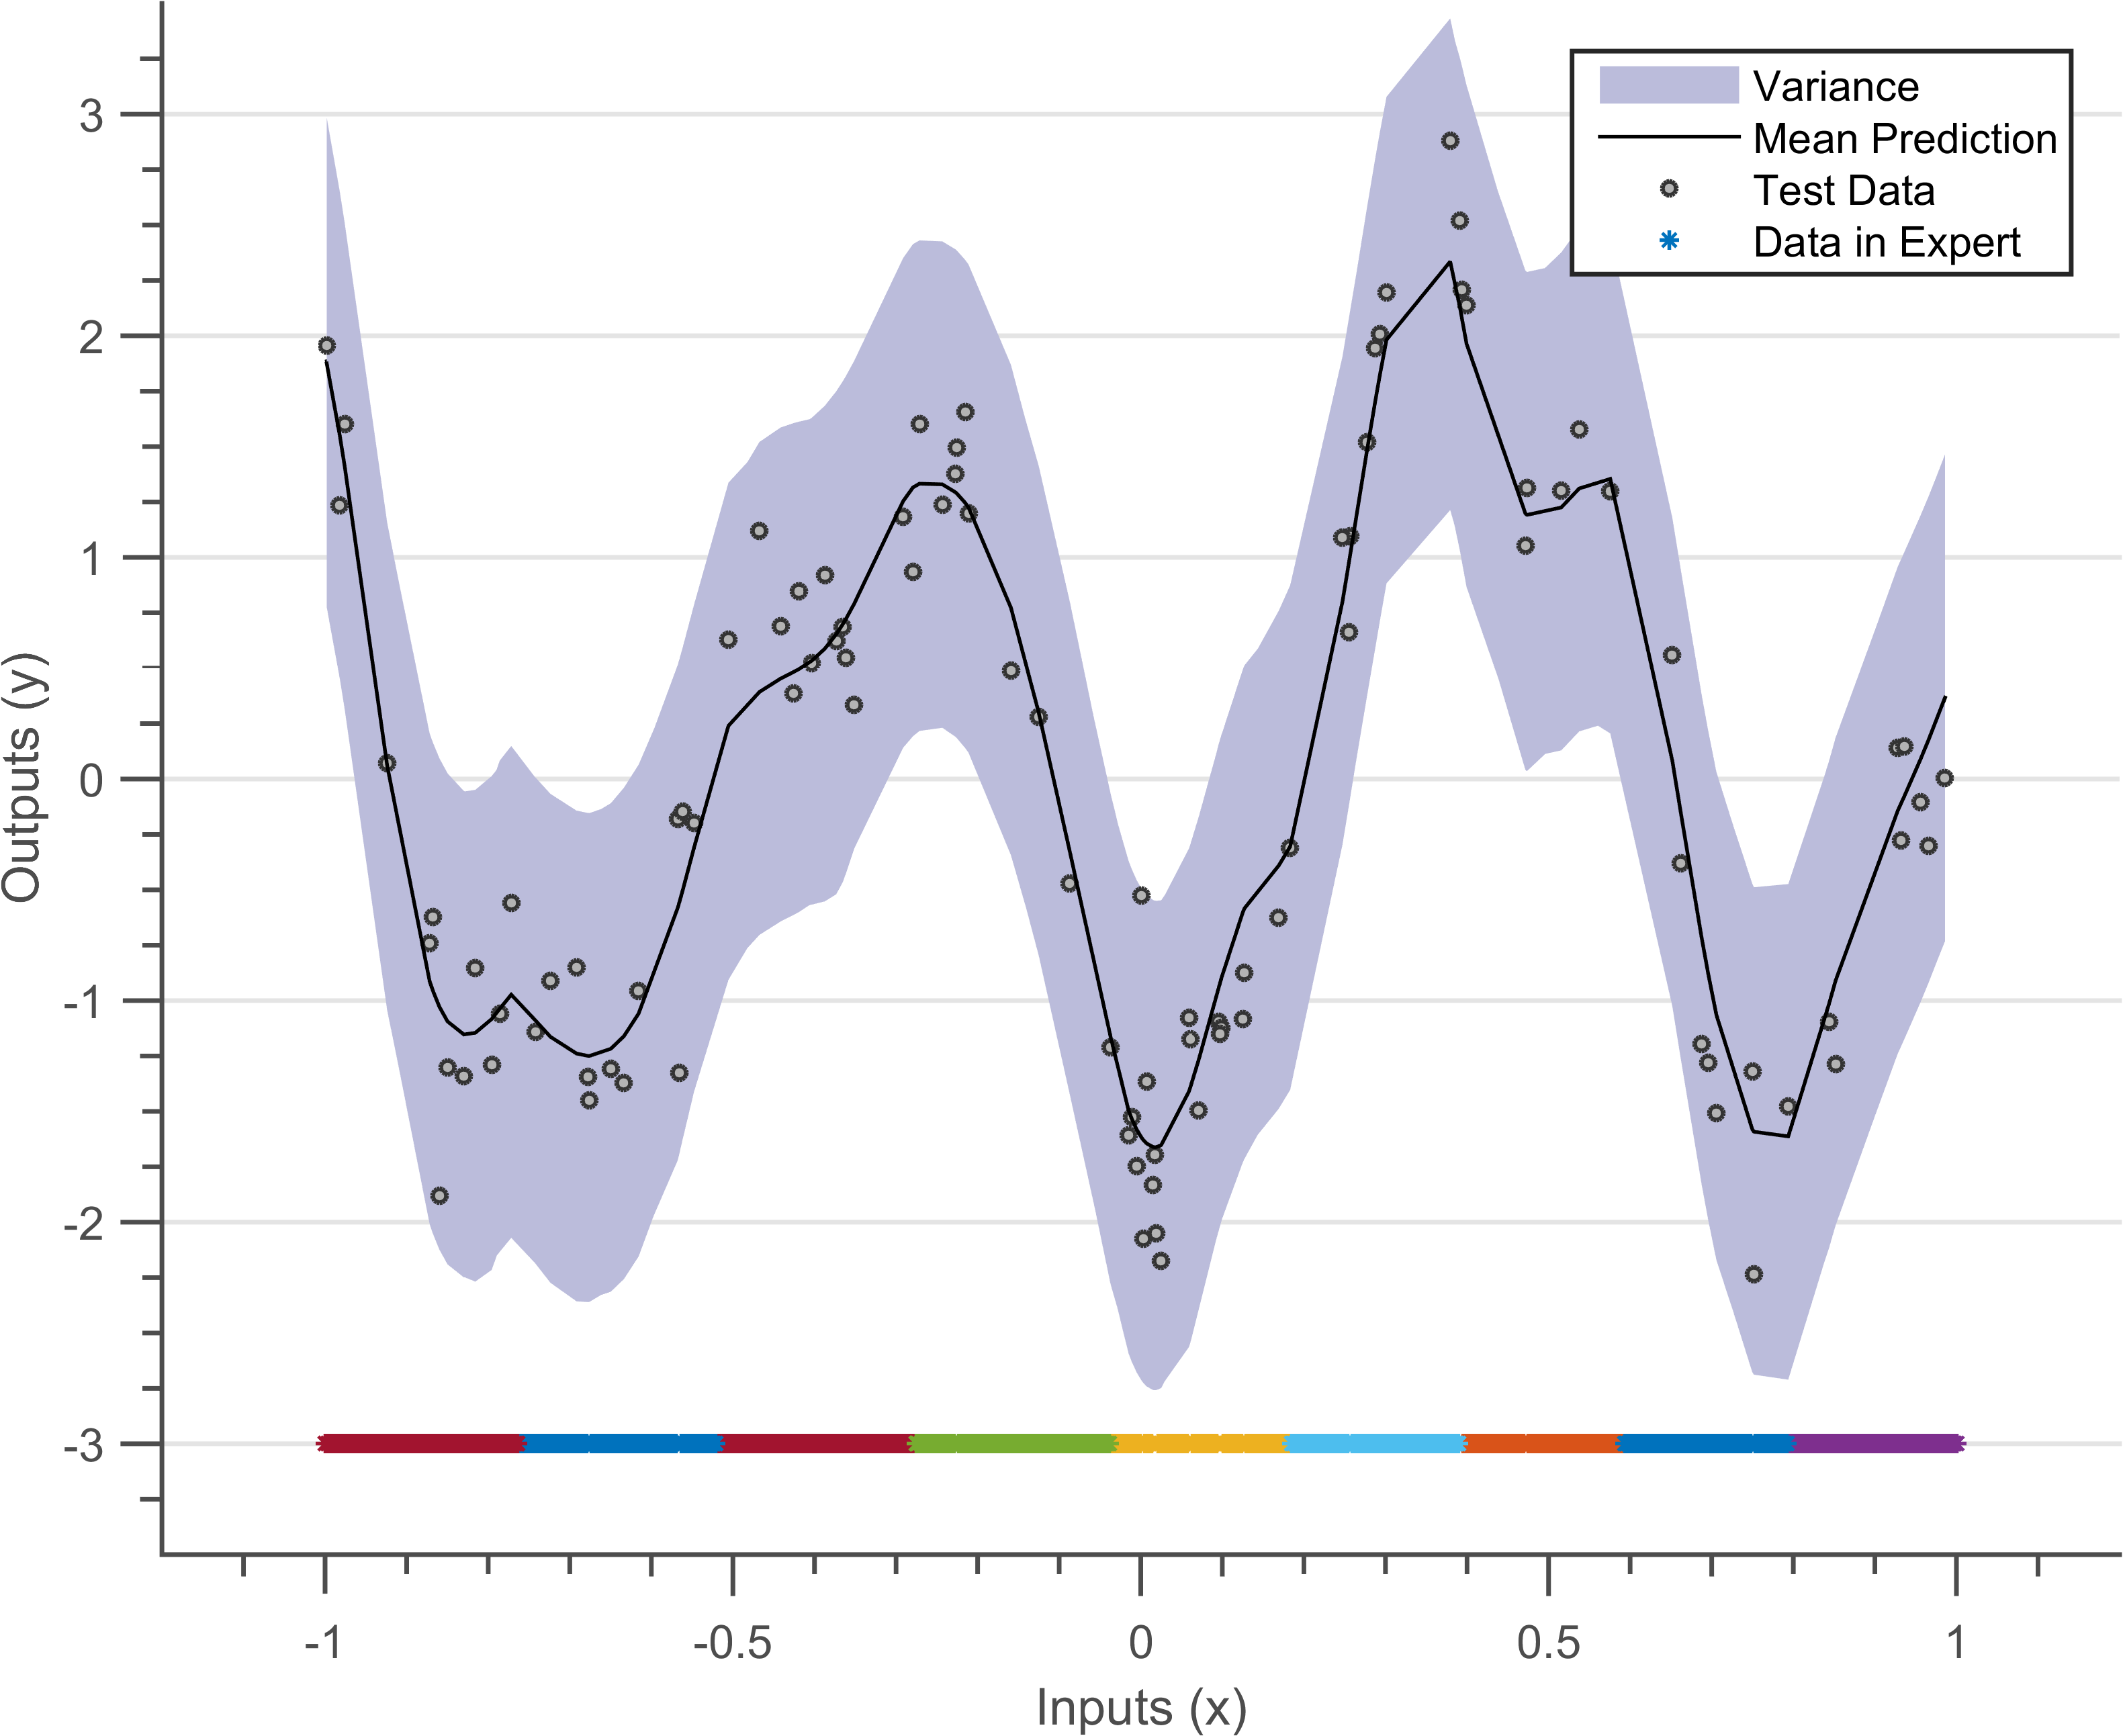
\includegraphics[width=0.45\textwidth]
        {images/part1/predictionOfm10_243}
        \label{predictionOfm10_243}
  }\quad
\subfigure[{10-fold RMSE box-plots for different number of points across. The box-plots in red are cases when only the hyper-parameters when the points are distributed using k-means clustering. The box-plots in blue are the cases when points are distributed randomly. The accuracy of prediction improves with increasing number of points in an expert}]
  {
        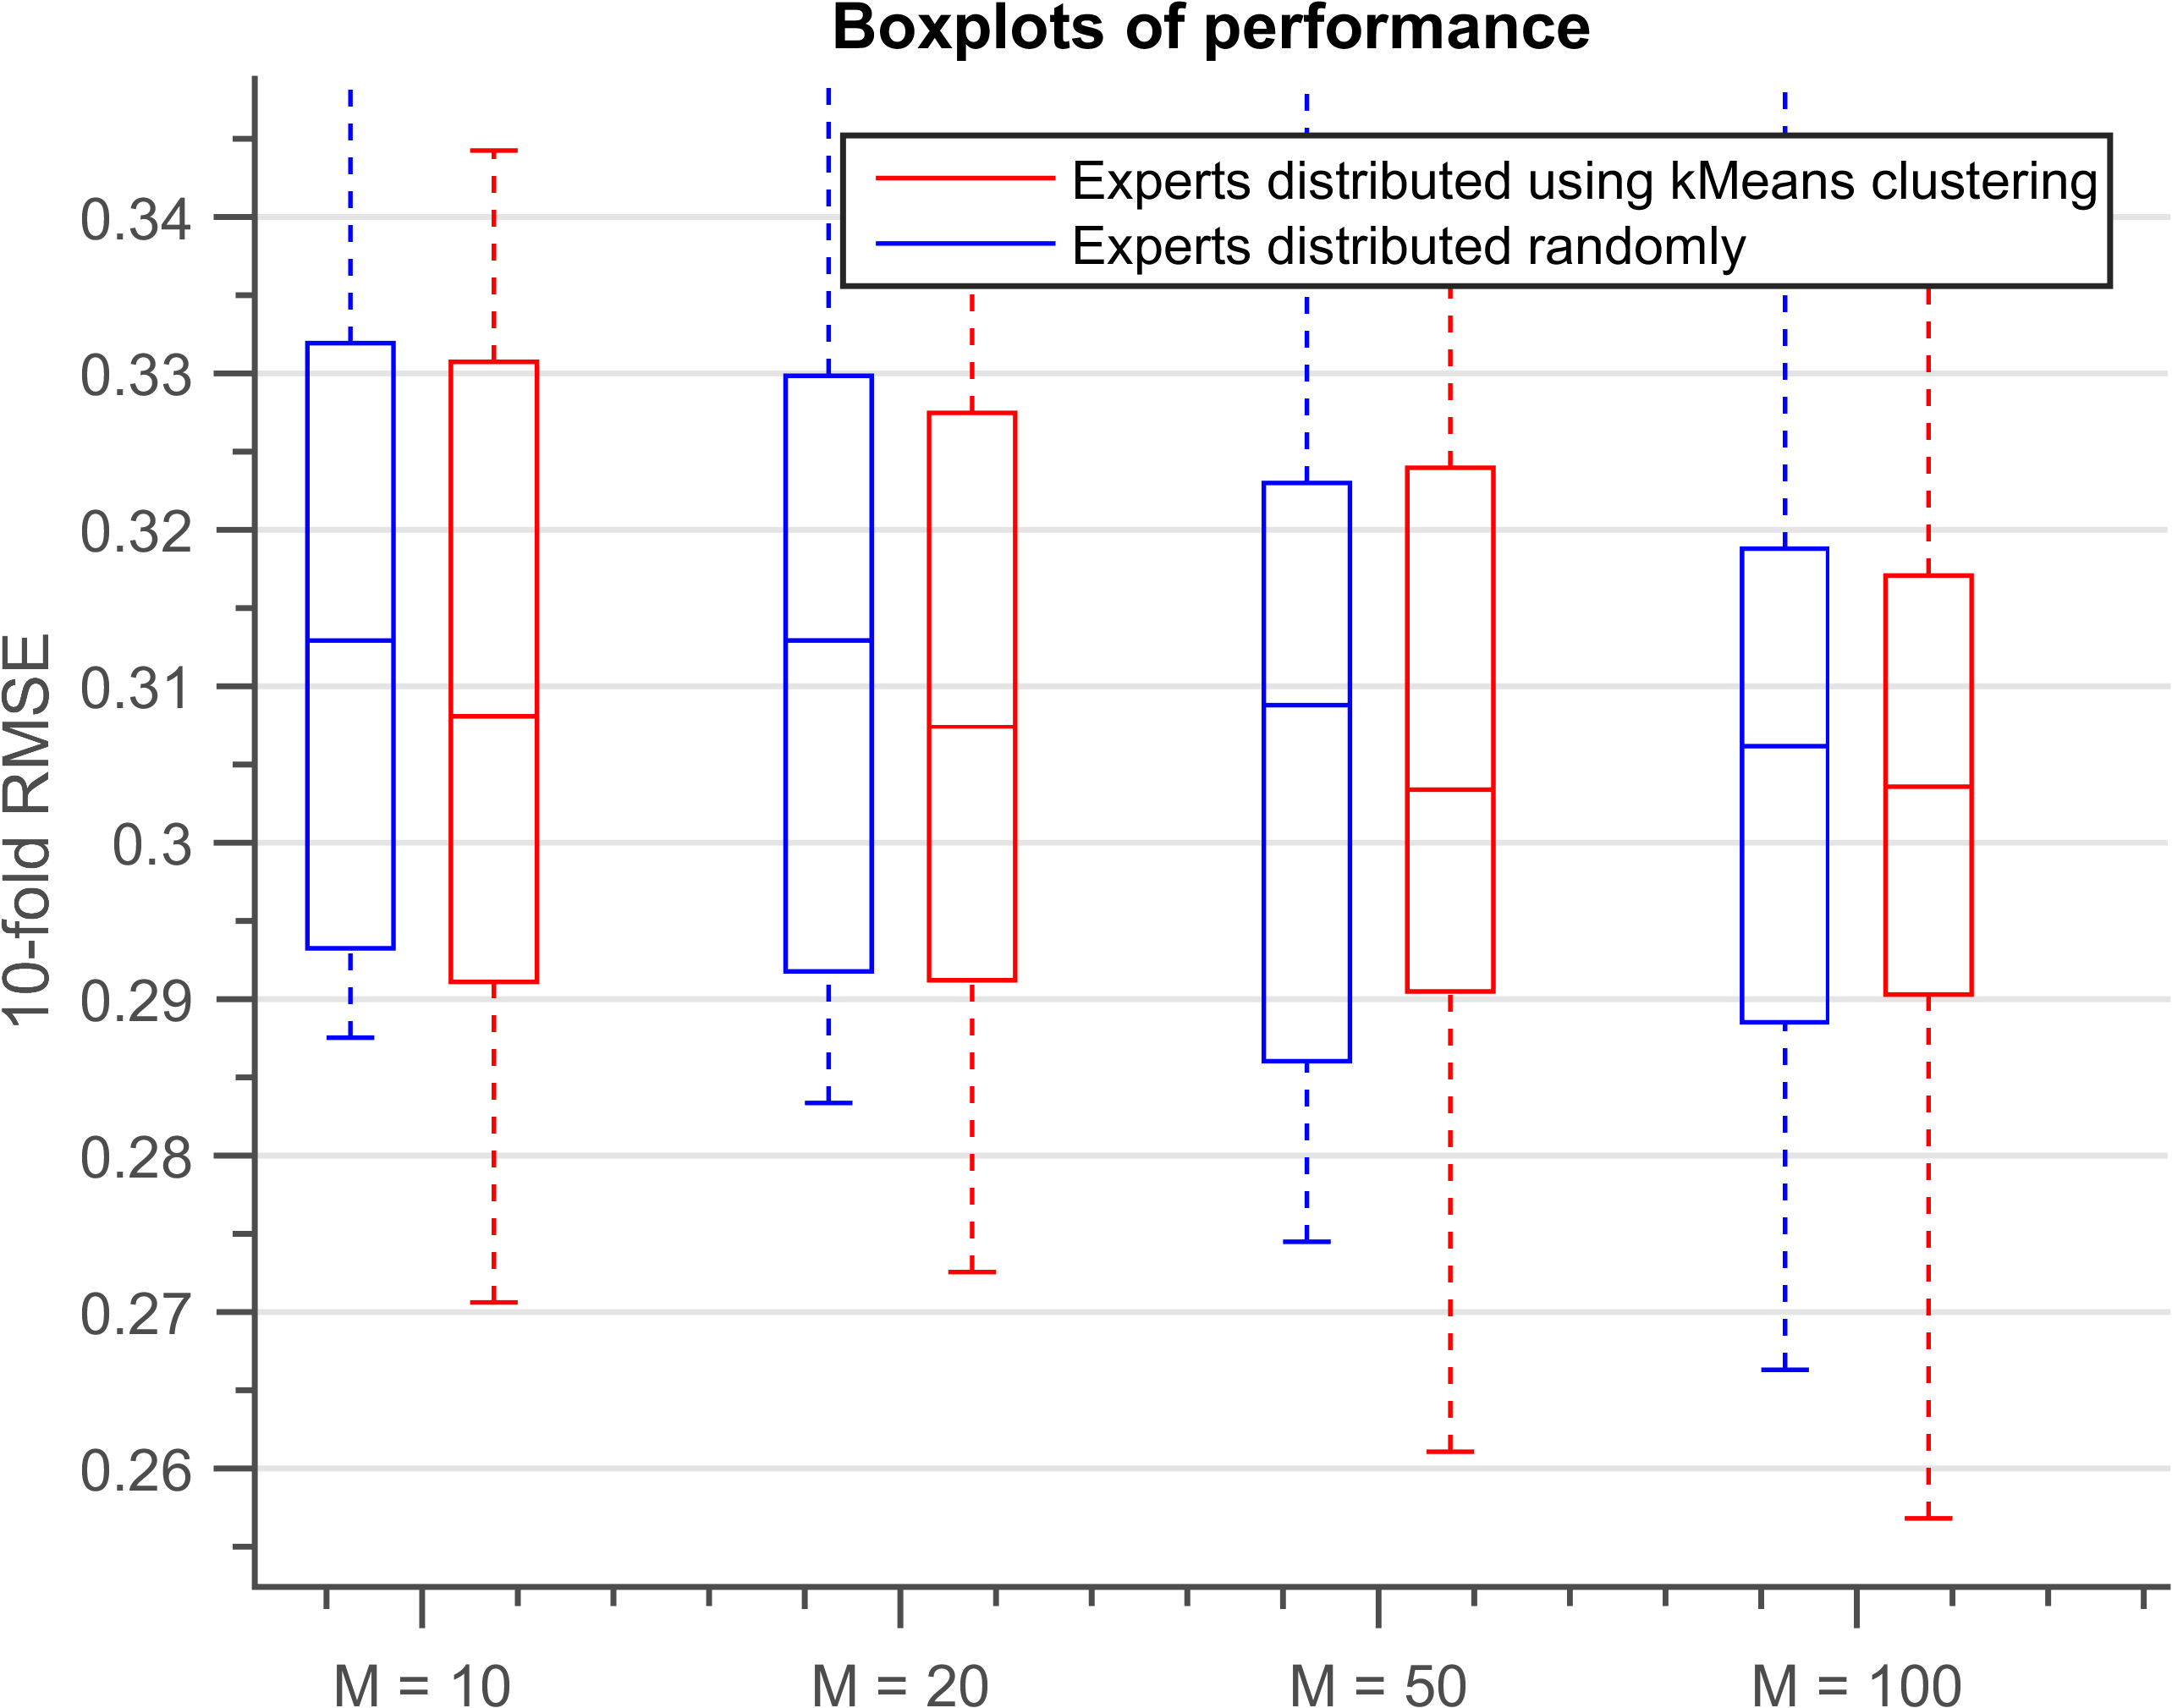
\includegraphics[width=0.45\textwidth]
        {images/part1/boxPlotsOfPerformance_243}
        \label{boxPlotsOfPerformance_243}
  }\quad
  
       \caption{Results of distributed GP Approximation on a toy-data set of size $N= 1000$}\label{figGPPredictionDistributed}
\end{figure}

\section{Summary and discussion}
The calculation of posterior in GPs becomes computationally intractable for large data sets. Calculating the precision matrix is an operation of computational complexity $\mathcal{O}(N^{3})$, putting a limit of $N \sim 10^4$ data points for model building. This chapter describes the state of the art for scaling up GPs for regression tasks. There exist two methods to scale up GPs, the first called sparse methods, they use a set of inducing inputs to reduce the computational cost of calculating the precision matrix. The second called distributed GP they divide the data set into smaller subsets called experts, distributing the model building into several batches. 

Sparse methods use Nystr\"{o}m approximation rewriting the Gram matrix as equation \ref{subSecSamplingFunctionsGPPrior}, thereby reducing the computational complexity to $\mathcal{O}(NM^{2})$ (M $\ll$ N), $M$ being the number of inducing points. Through experiments on a toy-dataset, it can be shown that we can set $M \sim N/10$ when inducing points are randomly distributed, and $M \sim N/50$ when the locations of inducing points are optimized. This approximation pushes the limit of GP Regression to $N \sim 10^6$ data points. Distributed GPs distribute the GP Regression tasks into several batches, thereby reducing the computational complexity to $\mathcal{O}(NP^{3})$ (P $\ll$ N), $P$ being the number of points in an expert. Through experiments on a toy-dataset we demonstrate that $P \sim N/100$ does not effects the regression task significantly. In fact we can further reduce $P$ if we enable repetition of points between experts. This enables to scale GPs to any number of data-points.

There are several reasons why GPs should be preferred to perform regression tasks. GPs provide a probabilistic framework to define a family of functions, while the covariance functions allows to incorporate a wide range of assumptions (part \ref{partIncorporatePattern}). GPs are computationally tractable, given a covariance function and observations, the predictive distribution can be calculated exactly. By providing a closed form expression of marginal likelihood GPs provide a powerful method to automatically select hyperparameters. Although GPs suffer in presence of large data sets, there exist several approximate methods to scale GPs to millions of data points. 

During the detailed design phase of an aircraft design cycle, high-fidelity code is used to explore the design space. This code is costly, mostly due to fine granularity of the meshes used. If we wish to use a surrogate model to explore the design space, then that surrogate model should be able to handle the large number of mesh points. Thankfully, due to the methods described in the current chapter we can scale GP regression to $N \sim 10^6$. We will demonstrate this by running a GP regression on millions of data-points in a CFD mesh. This surrogate model was used in a recent Airbus flight test campaign to compare pressures predicted from a high-fidelity CFD computation to pressures measured on the wing, in real time.

